\documentclass[12pt, letterpaper]{drexelthesis}
\usepackage{graphicx}% needed for including graphics e.g. EPS, PS
\usepackage{subfigure}% subcaptions for subfigures
\usepackage{subfigmat}% matrices of similar subfigures, aka small mulitples
\usepackage{afterpage}
\usepackage{dcolumn}%   decimal-aligned tabular math columns
	\newcolumntype{d}{D{=}{=}{4,4}}
\usepackage{amssymb}
%\usepackage[square, comma, sort&compress]{natbib}
\usepackage[square,sort,comma,numbers,sort&compress]{natbib}
%\usepackage[square]{natbib}
\usepackage{ifthen}
\usepackage{rotating}
\usepackage{lipsum}% http://ctan.org/pkg/lipsum
\usepackage{changepage}   % for the adjustwidth environment




\usepackage{tikz}
\usepackage{flushend}
\usepackage[algoruled,vlined,linesnumbered]{algorithm2e}
\usepackage{graphicx}        % standard LaTeX graphics tool
\usepackage[TABTOPCAP]{subfigure}
\usepackage{enumerate}
\usepackage{fancybox}
%added two new packages
\usepackage{amssymb}
\usepackage{amsmath}
\usepackage{lettrine}
%\usepackage{hangul-ucs/dhucs/tex-latex-dhucs/dhucs}
%\usepackage{hangul}
\usepackage{longtable}


\usetikzlibrary{arrows}
\usetikzlibrary{positioning}



\usepackage[linkbordercolor={1 1 1},citebordercolor={1 1
  1},urlbordercolor={0.0 0.0
  0.0},urlcolor=blue,colorlinks=true,linkcolor=black,citecolor=black]{hyperref}
\usepackage[squaren]{SIunits}
\usetikzlibrary{matrix,calc,shapes}
\usepackage{fancyhdr}

\definecolor{nodecolor}{RGB}{238,232,170} % light goldenrod
\definecolor{bgcolor}{rgb}{0.9,0.9,1.0} % light blue
\definecolor{sectcolor}{rgb}{0.0,0.0,0.5} % dark blue


%\newenvironment{danindent}{\begin{adjustwidth}{2cm}{}}{\end{adjustwidth}}




\tolerance=300

\author{Daniel Marc Lofaro}
\degreecollege{Doctor of Philosophy}
\degreearea{Electrical and Computer Engineering Engineering}
\advisor{Paul Oh}
\title{Control Architecture for High Degree of Freedom Complex Systems}
\gmonth{June}
%\gyear{2006} % default year is the current year

%\includeonly{chapter1}

%% for chapter heading
\usepackage{fancyhdr} 

\pagestyle{fancy} 
  \renewcommand{\chaptermark}[1]{                               
  \markboth{\thechapter{} #1}{}
  } 
  \fancyhf{} 
  \fancyhead[L]{\leftmark} 
  \fancyhead[C]{} 
  \fancyhead[R]{Page \thepage}
  \renewcommand{\headrulewidth}{0.4pt}
  \fancypagestyle{plain}{%
  }



\begin{document} 



	\doublespacing
	\maketitle 
\begin{preliminary}
	\sloppy
	\copyrightpage
	\include{dedications}
	\include{acknowledgments}
	\Large
\centering
Acronyms\\
\normalsize
\begin{tabular}{l | l}
\hline
AI & Artificial Intelligence\\
\hline
AIO & Asynchronous Input Output\\
\hline
CAD & Computer Aided Design\\
\hline
CAN & Controller Area Network \\
\hline
DARPA  &  Defense Advanced Research Projects Agency\\
\hline 
DH & Denavit–Hartenberg \\
\hline
DOF & Degree of Freedom \\
\hline
DRC  & DARPA Robotics Challenge \\
\hline
EEF  & End Effector\\
\hline
FIFO & First In, First Out\\
\hline
FK & Forward Kinematics\\
\hline
HRI & Human Robot Interaction\\
\hline
HOL & Head of Line\\
\hline
IK & Inverse Kinematics\\ 
\hline
IO & Input Output\\
\hline
IPC & Inter Process Comunication \\
\hline
JMC & Joint Motor Controller\\
\hline
KAIST & Korea Advanced Institute of Science and Technology \\
\hline
MPI & Message Passing Interface\\
\hline
MIRR & Major Research Infrastructure Recovery and Reinvestment\\
\hline
MLB & Major League Baseball\\
\hline
NSF & National Science Foundation \\
\hline
PID & Proportional Intergral Deritive\\
\hline
POSIX & Portable Operating System Interface\\
\hline
RT & Real-Time\\
\hline
ROS & Robot Operating System\\
\hline
SRM & Sparse Reachable Map \\
\hline 
ZMP & Zero Moment Point\\
\hline
\end{tabular}

	\chapter{Hubo Joint Acronyms}
\Large
%%\centering
\begin{center}
Hubo Joint Acronyms\\
\normalsize
\begin{longtable}{c | l || c | l}
\hline
		RHY				&	Right Hip Yaw     & RHR				&	Right Hip Roll \\
		\hline
		RHP				&	Right Hip Pitch   & RKN				&	Right Knee Pitch\\
		\hline
		RAP				&	Right Ankle Pitch & RAR				&	Right Ankle Roll\\
\hline

\hline
		LHY				&	Left Hip Yaw      & LHR				&	Left Hip Roll\\
		\hline
		LHP				&	Left Hip Pitch    & LKN				&	Left Knee Pitch\\
		\hline
		LAP				&	Left Ankle Pitch  & LAR				&	Left Ankle Roll\\
\hline
& & & \\
\hline
		RSP				&	Right Shoulder Pitch & RSR			&	Right Shoulder Roll\\
		\hline
		RSY				&	Right Shoulder Yaw   & REB			&	Right Elbow Pitch\\
		\hline
		RWY				&   Right Wrist Yaw      & RWR			&   Right Wrist Roll\\
		\hline
		RWP				&   Right Wrist Pitch    & & \\
\hline

\hline
		LSP				&	Left Shoulder Pitch  & LSR		    &	Left Shoulder Roll\\
		\hline
		LSY				&	Left Shoulder Yaw    & LEB			&	Left Elbow Pitch\\
		\hline
		LWY				&   Left Wrist Yaw       & LWR			&   Left Wrist Roll\\
		\hline
		LWP				&   Left Wrist Pitch	 & & \\
\hline
& & & \\
\hline
		NK1				& Neck 1    & NKY				& Neck Yaw\\
		\hline
	    NK2				& Neck 2    & WST				& Trunk Yaw \\
\hline

		  & & \\
\hline
		RF1				&	Right Finger 1 & RF2				&	Right Finger 2\\
		\hline
		RF3				&	Right Finger 3 & RF4				&	Right Finger 4\\
		\hline
		RF5				&	Right Finger 5 & & \\
\hline

\hline
		LF1				&	Left Finger 1 & LF2				&	Left Finger 2\\
		\hline
		LF3				&	Left Finger 3 & LF4				&	Left Finger 4\\
		\hline
		LF5				&	Left Finger 5 & & \\
		
\end{longtable}
\end{center}
	\Large
\centering
Symbols\\
\normalsize
\begin{tabular}{l | l | l}
\hline
Symbol     & Definition                                                         & Units \\
\hline
$L$        & Filter buffer length                                               & $N/A$\\
\hline
$N$        & Discrete time step                                                 & $sample$\\
\hline
$T$        & Period                                                             & $sec$ \\
\hline
$\theta_a$ & Actual position of joint as measured from the encoders             & $rad$ \\
\hline
$\theta_c$ & Reference set to the actuator                                      & $rad$ \\
\hline
$\theta_d$ & Desired Reference before being set to Hubo-Ach FeedForward Cahnnel & $rad$ \\
\hline
$\theta_e$ & Actuiator PID error                                                & $rad$ \\
\hline
$\theta_r$ & Desired reference on the Hubo-Ach FeedForward Channel              & $rad$ \\
\hline
$\alpha$   & Rotation about the x-axis (roll)					& $rad$ \\
\hline
$\beta$    & Rotation about the y-axis (pitch)                                  & $rad$ \\
\hline
$\gamma$   & Rotation about the z-axis (yaw)                                    & $rad$ \\
\hline

\end{tabular}

	
  \centering
      \includegraphics{./qrcode/qrcode-phd.png}\\
      Video: http://danlofaro.com/phd/ \\
If you see the image above use a \textbf{QR-Code reader} or enter the URL listed above to see the digital content.  The digital content usually consists of videos or interactive demonstrations.


%%	\include{dedications}
%%	\include{acknowledgments}
	\mytableofcontents
	\mylistoftables
	\mylistoffigures
%%	\begin{center}
\large\bf{Abstract:}
\end{center}
\normalsize

\bf{
\noindent The degrees of freedom (DOF) of robots and complex systems have been increasing increasing exponentially since the early 20th century.
Today it is common place for complex control systems to have 40 DOF. 
This number is projected to be 70 DOF by the year 2020.
Robots with high DOF allows for complex tasks such as tool manipulation, greater human-robot interaction and agile full-body locomotion.
More DOF require greater attention to local communication delays, bandwidth, system configuration and stability.
In addition different tasks being performed by separate parts of the robot in tandem bring on greater issues including controller timing and priorities.
The increase in DOF on single system requires that the traditional methods of controller design be re-examined.

\noindent This dissertation describes a Unified Algorithmic Framework for High Degree of Freedom Complex Systems and Humanoid Robots that allows a user to develop controllers using a three tier infrastructure.
The Unified Algorithmic Framework called Hubo-Ach is a multi-process based system that allows for robust multi-rate simultaneous control and seamless implementation between virtual, miniature, and full-size robots with no modification.
The three tier infrastructure provides different levels of cost to entry and testing.
Examples of this field tested framework functioning on simulated, miniature, and full-size high DOF robots is given as well as validation by external researchers.
}




\end{preliminary}

\begin{thesis}
	\fussy
	\chapter{Introduction}
%%------ Intro -------%%
	Since 2005  
Creating controllers for high degree of freedom complex systems is essential for development of the next generation of robots.
Due to the inherent complexity and often high expense of the system, controllers must be able to be tested.



It is common place for a complex electrical mechanical system to have multiple different controllers running in tandem.  
Different controllers are needed when the system is in different states or doing different tasks.
Combining these controllers is a problem in complex system.
This problem is hard when each controller has different frequencies, timing requirements (asyncronous vs. syncronous), latency restrictions, newest state data ie smore important then older state data and most basic of all languages the controller is written in.
This is especially true for complete and complex autonomous systems.
I define a complete and complex autonomous system as an electro mechanical mechanism with high degree of freedom (DOF) that is capable of making its own decisions through the use of sensor data processed by its artificial intelligence (AI).
The combination of high DOF and the requirement for autonomy makes the work space broad and controllers complex.
The overarching question becomes; What is the control system structure for a complete and complex autonomous systems with high DOF, a multitude of sensors, AI performing high-level and low-level tasks all while keeping a stable system structure conducive to collaborative work?
Current methods of solving the problem of controller synchrony and latest state data is to keep your critical control elements in the primary control loop.
Inter-process communication (IPC) and/or network sockets to communicate between the high level and low level processes even if written in different languages.
The majority of IPC have the problem of \textit{head of line} blocking (HOL) which means you must read the older data in a buffer before you read the newest data.
In the computer science field this is not a problem because all data being intact is typically desired.  
In the field of robotics and control the most recent state data is more important to a real-time control system to act on.
This thesis shows that by expanding on the idea of multi-process controllers connected to high-speed low-latency IPC you can create a \textit{robot layer} on a computer platform that will allow low-level controllers to run in separate processes while still allowing them access to the most recent data as the priority.
The new technical idea is the \textit{robot layer}, a control layer that allows external processes to run like normal and not deal with the specifics of the given robot system.
The robot system can be replaced by a simulated system without any of the processes needing to be modified or even know of the change.
This allows more mature controllers to be easily interfaced with this system without modifying control rates or timing.
This \textit{robot layer} must be:
\begin{itemize}
\item Have a IPC latency much less then that of the robot's inherent sampling period $t_{ipc}<<T_{r}$
\item Allow for command rates much slower then the inherent sampling period $T_{slow}>>T_{r}$
\item Allow for command rates much faster then the inherent sampling period $T_{fast}<<T_{r}$
\item Allow for arbitrary command rates.
\item Allow for real-time and non-real-time controllers to command actuators
\item Allow for all processes to have access to the newest data first
\item Allow for no more then one rt time step delay between command and robot actuator retrieval
\item Commanded such that it is for an arbitrary robotic actuator.
\item Triggering for process synchronization
\item Triggering for simulator synchronization and holding
\end{itemize}
We can succeed now not only because the bleeding edge technology allows for the fast enough communication between processes with access to the latest data.

Results are measured quantitatively and qualitatively.
Data showing proper loop rates, timings, controller implementation, simulation connections etc. show the viability of the system.
User survey shows methodology is sound, useful, and practical.





My Thesis shows is that a multi-process control structure coupled with the proper timing mechanisms is conducive to answering these questions.
It is shown with physical experiments and the creation of Hubo-Ach\cite{lofaroRAM2013}; a fully functional Sim-Time and Real-Time control system for complete and complex autonomous systems.

Through experimentation I prove my control system is a viable way of controlling complete and complex autonomous system and still be conducive to collaborative work.  
A road map of how my research has taken me to my thesis is shown in Section~\ref{sec:roadmap}.
As proof of viability I show the basic structure of my system \textit{Hubo-Ach} in Section~\ref{sec:hubo-ach}.  
I give step by step examples in Section~\ref{sec:simpleExamples}.
Section~\ref{sec:simulator} shows how we can move from real-time to using a simulated version of the platform in simulation time without having to change the controller.
Section~\ref{sec:task} describes the experiment which consists of making the robot preform an advanced task that pulls together visual, kinematic, path planning and other controllers together using this one system.
The techniques used stem from my contributions in Section~\ref{sec:contributions}.
Section~\ref{sec:results} shows the results of the experiment thus show the viability of the system.
Lastly Section~\ref{sec:conclusion} discusses the results of the work and the future of this system.

Before I continue it is important to note that my work has already been validated by my pears because:
\begin{itemize}
\item It was chosen to be the primary control system for the DARPA Robotics Challenge Track-A Team DRC-Hubo, Section~\ref{sec:drc}.
\item It is being used in the NSF-MIRR project\footnote{NSF-MIRR: Major Research Infrastructure Recovery and Reinvestment (MIRR) \#CNS-0960061 sponsored by the the U.S. National Science Foundation (NSF)}.
\item It is currently being used by MIT, WPI, Purdue, Ohio State, Swarthmore College, Georgia Tech, and Drexel University.
\end{itemize}

For the remainder of this document the complete and complex autonomous systems that I will be referring to are robots.
The majority of examples given will be in reference to humanoid robotics and the Hubo2+ (KHR-4+) platform.
The Hubo platform is described in Section~\ref{sec:hubo}.







%%------ Path To Ph.D. -------%%	
	\section{Motivation}\label{sec:roadmap}	
		This section provides context to the origin of the idea of a unified algorithmic framework for complex systems.

%%%%%%% Put what I wrote here
\begin{figure}[thpb]
  \centering
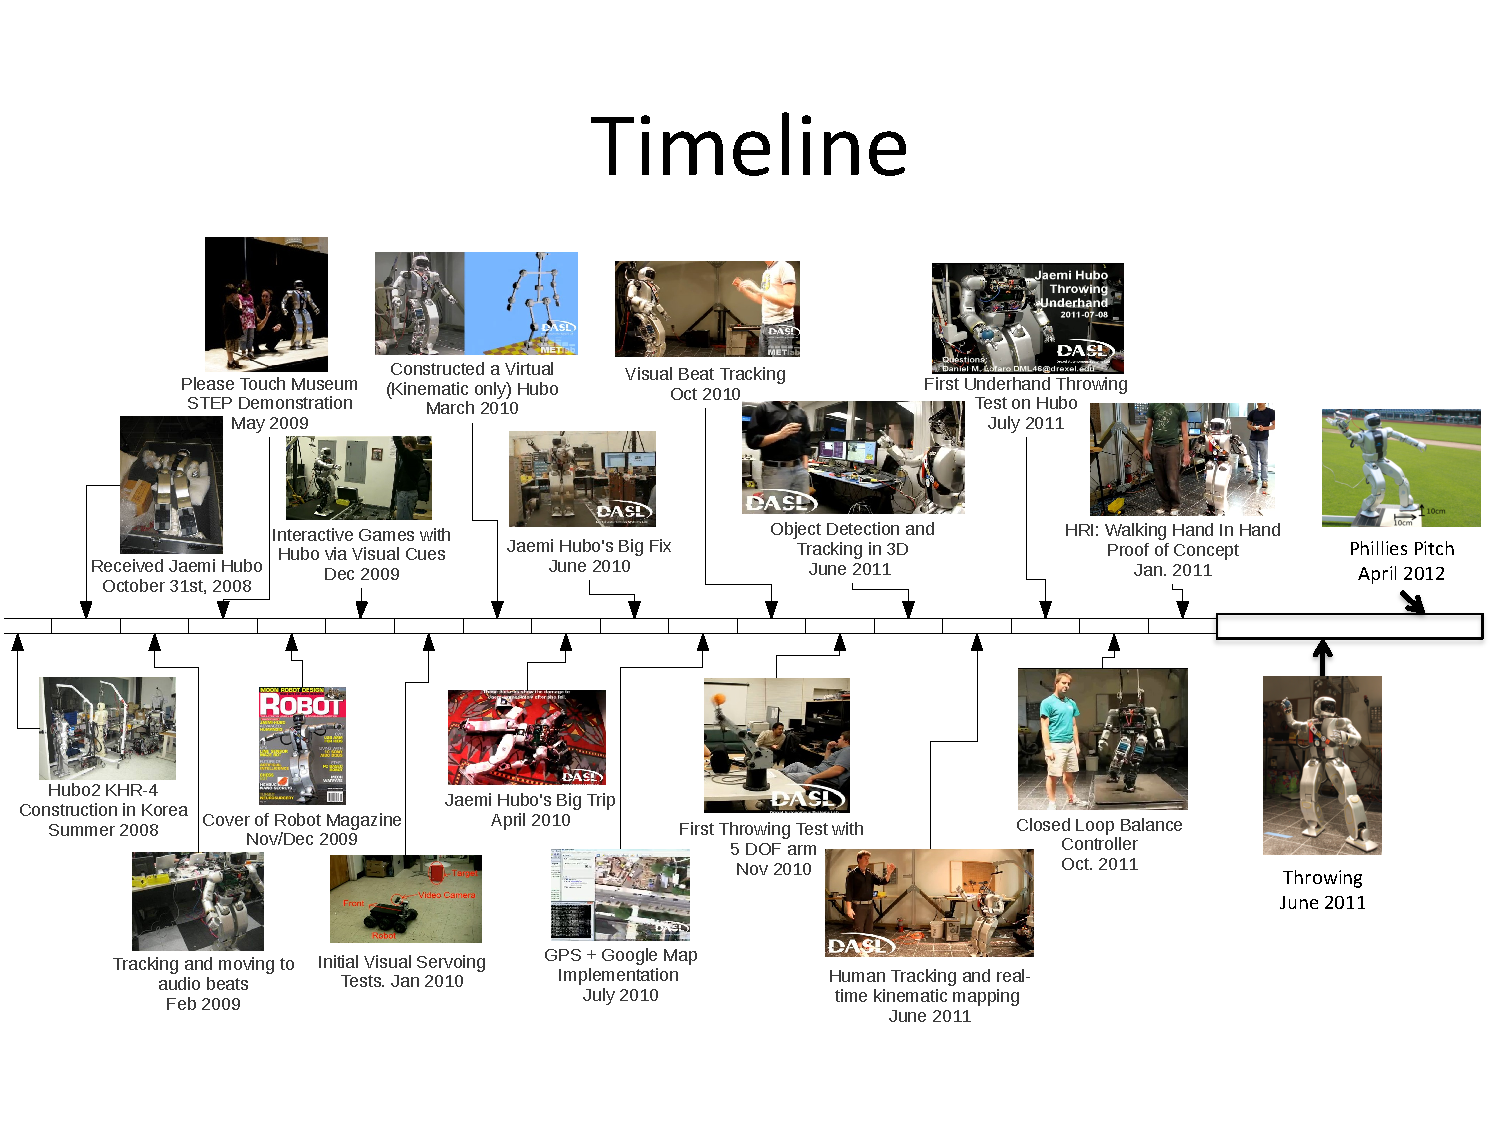
\includegraphics[angle=90, width=0.9\columnwidth]{./pix/Timeline.pdf}
  \caption{Timeline of Daniel M. Lofaro's research from 2008 to 2012}
  \label{fig:timeline}
\end{figure}

\subsection{Human Robot Interaction}
The initial goal was to have a humanoid robot become an interactive musical participant with humans.
This spawned the creation of a visual method of tracking the beat in the absence of auditory cues\cite{5686847}.
This came from a modification of a method of allowing children to play interactive games with humanoid robots\cite{lofaroGamesRobot}.
The resulting method was effective, but to increase the accuracy it was required to combine a pre-existing auditory beat tracker with the visual system.
This calumniated with a multi process system that combine the auditory and visual beat trackers\cite{lofaroIASTED2011,6094987,lofaroEURASIP2011}.
A human comparison was completed and found that this combined method was as accurate at detecting the beat in music as average humans.

\subsubsection{Results from preliminary experiments}
When collaborating with other to create a complex robot control systems integrating controllers is difficult because of the use of:
\begin{itemize}
\item different loop rates causing synchronization issues
\item different programming languages making using the same libraries a challenge
\end{itemize}

It was found that it is best to keep each working systems \textit{independent} allowing them to run at their native rate and on their native platforms\cite{ach}.



\subsection{High Degree of Freedom Kinematic Planning}
The next challenge was to perform kinematic planning for end effector velocity control. 
This resulted in the development of a method that is able to solve inverse kinematics (IK) for high degree of freedom (DOF) systems where there is no closed-form solution as well as create collision free trajectories for high DOF robots\cite{6385987}.
This is described in detail in Section~\ref{sec:srm} and \ref{sec:baseball}.
This culminated in the verification and validation of the system by an experiment where Hubo full-size humanoid robot throw the first pitch at a Major League Baseball (MLB) game\cite{lofaroHumanoids2012,6462956}.

\subsubsection{Results from preliminary experiments}
As best practice when controllers and planners are implemented it is important that low-level controllers such as balance and obstacle avoidance run at all times\cite{lofaroRAM2013}. 
Non-priority controllers such as throwing trajectory planning can run in the background in a separate process.
Keeping the processes separate allowed the system to be more resistant to lag and crashes of one or more of the controllers.
This brought validation to the overarching plan for the unified algorithmic framework for complex systems and humanoid robots.




\subsection{Lessons Learned}

At this point creating these experiment it was required to \textit{hacked} together pre-existing systems that allowed the robot to do the task.
This is the point where it was realized that a \textit{unified algorithmic framework for complex systems and humanoid robots} was required for further development in the field.
Key lessons learned from these experiments were:
\begin{itemize}
\item Must inherently decouple controllers loop rates and phases
\item Must allow for collaborators not have to \textit{inject} their code into existing source.
\item Must work with multiple robots for testing, evaluation, validation, and verification.
\end{itemize}

\noindent This is where Hubo-Ach was born.
The idea was to create a multi process architecture for humanoid control using state of the art high-speed low-latency Inter-Process Communication (IPC) techniques\cite{lofaroRAM2013}.
This is different from traditional IPC techniques because of the lack of head of line (HOL) blocking and focus on low-latency.
Section~\ref{sec:ipc} gives further details and comparisons of different IPCs.


The need for this unified framework was amplified when the Hubo was chosen to be the primary platform for the DRC-Hubo\footnote{DRC-Hubo: http://www.drc-hubo.com/} Track-A team.
Since its initial conception Hubo-Ach has become a fully functional system used in active research by multiple universities including MIT, WPI, Purdue, Ohio State, Swarthmore College, Georgia Tech, and Drexel University\cite{lofaroTePRA2013HuboAch,lofaroTePRA2013Valve}.
This research also acts as a key source of verification and validation of the system.



%%------ About Hubo -------%%
	\section{Platforms}\label{sec:robots}
	This section describes the different platforms that are focused on in this document.
		\subsection{Hubo2 Plus}\label{sec:hubo}
			%\subsubsection{Hubo2 Plus}
The Hubo2+ is a $1.3\meter$ (4' 3'') tall, 42 $kg$ (93 $lb$) full-size
humanoid robot.  The Hubo series was designed and constructed by the
Korean Advanced Institute of Science and Technology (KAIST) and
spinoff Rainbow Inc. \cite{hubofirst}.  It has 38 degree of freedom:
six per arm and leg, five per hand, three in the neck, and one in the
waist.  Sensors include three-axis force-torque sensors in the wrists
and ankles, accelerometers in the feet, and an inertial measurement
unit (IMU).  The sensors and embedded motor controllers are connected
via a Controller Area Network to a pair of Intel Atom PC104+ PCs
running a GNU/Linux distribution.



% The reference commands for
% all of the joints are sent from the primary control computer (x86) to
% the individual motor controllers via two Controller Area Network (CAN)
% buses.  This is the same communications bus found in most modern motor
% vehicles.  There are currently eight Hubo's functioning in the United
% States as of December 2012.  Four reside at Drexel University and one
% at Georgia Tech, Purdue, Ohio State and MIT.  Jaemi Hubo is the oldest
% of the Hubos in America and has been at the Drexel Autonomous Systems
% Lab\footnote{Drexel Autonomous Systems Lab:
%   http://dasl.mem.drexel.edu/} (DASL) since 2008 \cite{jaemiHuboSRM}.
% Fig.~\ref{fig:hubo} shows the major dimensions of Hubo.

% \begin{figure}[thpb]
%   \centering
% \includegraphics[width=1.0\columnwidth]{./pix/huboSkel.pdf}
%   \caption{Hubo2 Plus platform: 38 DOF, 130 $cm$ tall full-size humanoid robot weighing 37 $kg$.}
%   \label{fig:hubo}
% \end{figure}

% All joints of the major joints are high gain PID position
% controlled with the exception of the fingers.  The fingers are
% open-loop PWM controlled.
% The sensing capability consists of a three
% axis force-torque (FT) sensor on each leg between the end of the ankle
% and the foot as well as between the arm where it connects to the hand.
% Additionally it has an inertial measurement unit (IMU) at the center
% of mass and accelerometers on each foot.

%%% Local Variables:
%%% mode: latex
%%% TeX-master: "ach"
%%% End:

		\subsection{Mini-Hubo}\label{sec:mini-hubo}
			Mini-Hubo\cite{threeTier} is a miniture version of the Hubo platform discribe in Section~\ref{sec:hubo}.
It is used as the Test and Evaluation (T\&E) stage of the three tier infrastructure discribed in Section~\ref{sec:threeTier}.
Mini-Hubo is kinematically scaled to the Hubo platform.
The atrobutes of the Mini-Hubo system are in Table~\ref{table:huboMiniSensors}.
The robot is shown in Fig.~\ref{fig:mini-hubo}


\begin{table}
\centering
\caption{Mini-Hubo Platform Specifications}
\begin{tabular}{| l || l |}
\hline
Height      		& $46~cm$			\\
\hline
Weight			& $2.9~kg$			\\
\hline
DOF			& 22				\\
\hline
Joint Control Type	& PID Position			\\
\hline
Computer		& $1.6~Ghz$ Atom		\\
			& $2~Gb$ DDR2 RAM		\\
\hline
Operating System	& Debian Linux			\\
\hline
Battery			& $14.8V$ $3.2~Ah$ $30C$ LiPo	\\
\hline
Sensors			& 2x 3 Axis Force Torque	\\
\hline
Vision			& Monocular			\\
			& RGBD				\\
\hline
\end{tabular}
\label{table:huboMiniSensors}
\end{table}





\begin{figure}[thpb]
  \centering
\includegraphics[width=0.37\columnwidth]{./pix/mini-hubo.jpg}
  \caption{Mini-Hubo platform: 22 DOF, 46 $cm$ tall miniture-size humanoid robot weighing 2.9 $kg$.}
  \label{fig:mini-hubo}
\end{figure}

		\subsection{OpenHubo}\label{sec:openhubo}
			OpenHubo\cite{dlofaro-srm} is an open-source kinematic and dynamic simulator for the the Hubo2 and Hubo2+ series robots.
It was developed by the Drexel Autonomous Systems Lab and runs using the open-source robot simulation environment OpenRAVE\cite{diankovThesis}.
Fig.~\ref{fig:openhubo1} shows the OpenHubo model.
Table~\ref{table:huboOpenSensors} shows the spesifications of OpenHubo.


\begin{figure}[thpb]
  \centering
      \includegraphics[width=0.4\columnwidth]{./pix/hBody.png}\includegraphics[width=0.4\columnwidth]{./pix/hCol.png}
      
\caption{OpenHubo model of the Hubo2 humanoid robot developed by the Drexel Autonomous Systems Lab and runs using the open-source robot simulation environment OpenRAVE\cite{diankovThesis}.}
\label{fig:openhubo1}
\end{figure}


\begin{table}
\centering
\caption{OpenHubo Platform Specifications}
\begin{tabular}{| l || l |}
\hline
Dynamics      		& Yes (ODE)			\\
\hline
Kinematic		& Yes				\\
\hline
DOF			& 40				\\
\hline
Joint Control Type	& PID Position			\\
\hline
Computer		& $1.6~Ghz$ Atom		\\
			& $2~Gb$ DDR2 RAM		\\
\hline
Enviroment		& OpenRAVE\cite{diankovThesis}	\\

\hline
Sensors			& 1x 4 Axis IMU			\\
			& 4x 3 Axis Force Torque	\\
\hline
\hline
\end{tabular}
\label{table:huboOpenSensors}
\end{table}

		








%%------ Three Tier infrastructure -----%%
	\section{Three Tier Infrastructure}\label{sec:threeTier}
		The three tier infrastructure allows for:
\begin{itemize}
\item Rapid Prototype (RP) phase with zero cost to entry (OpenHubo Platform Section~\ref{sec:openhubo})
\item Test and Evaluation (T\&E) phase with low cost to entry (Mini-Hubo Platform Section~\ref{sec:mini-hubo})
\item Verify and Validate (V\&V) phase with lease-time cost to entry (Hubo Platform Section~\ref{sec:hubo})
\end{itemize}



The OpenHubo\cite{6385987} kinematic and dynamic model in OpenRAVE\cite{diankovThesis} is the RP for this document.
The T\&E phase is a miniature kinematically scaled structure to that of the Hubo platform.
Mini-hubo\cite{threeTier} acts as the model for the T\&E phase.
The Hubo platform\cite{4058572} is used as the full-size humanoid for this infrastructure.  
A key aspect is that a single controller commands all three of the phases.
This controller is called Hubo-Ach and is discribed in Section~\ref{sec:hubo-ach}.
Fig~\ref{fig:threeTier} shows the three tier infrastructure for the Hubo platform.

The key point of the three tier infrastructure is allowing for testing on the RP.
When the algorithms applied to RP works, moving to the T\&E phase is the next step.
If it does not work in T\&E then the cycle states movement back to the RP phase.
If it does work then movement to the V\&V phase is the next step.
If application to V\&V is not successful then the cycle states movement back to T\&E or RP phase.
If it does work then the project is complete \cite{threeTier}.

\begin{figure}[thpb]
  \centering
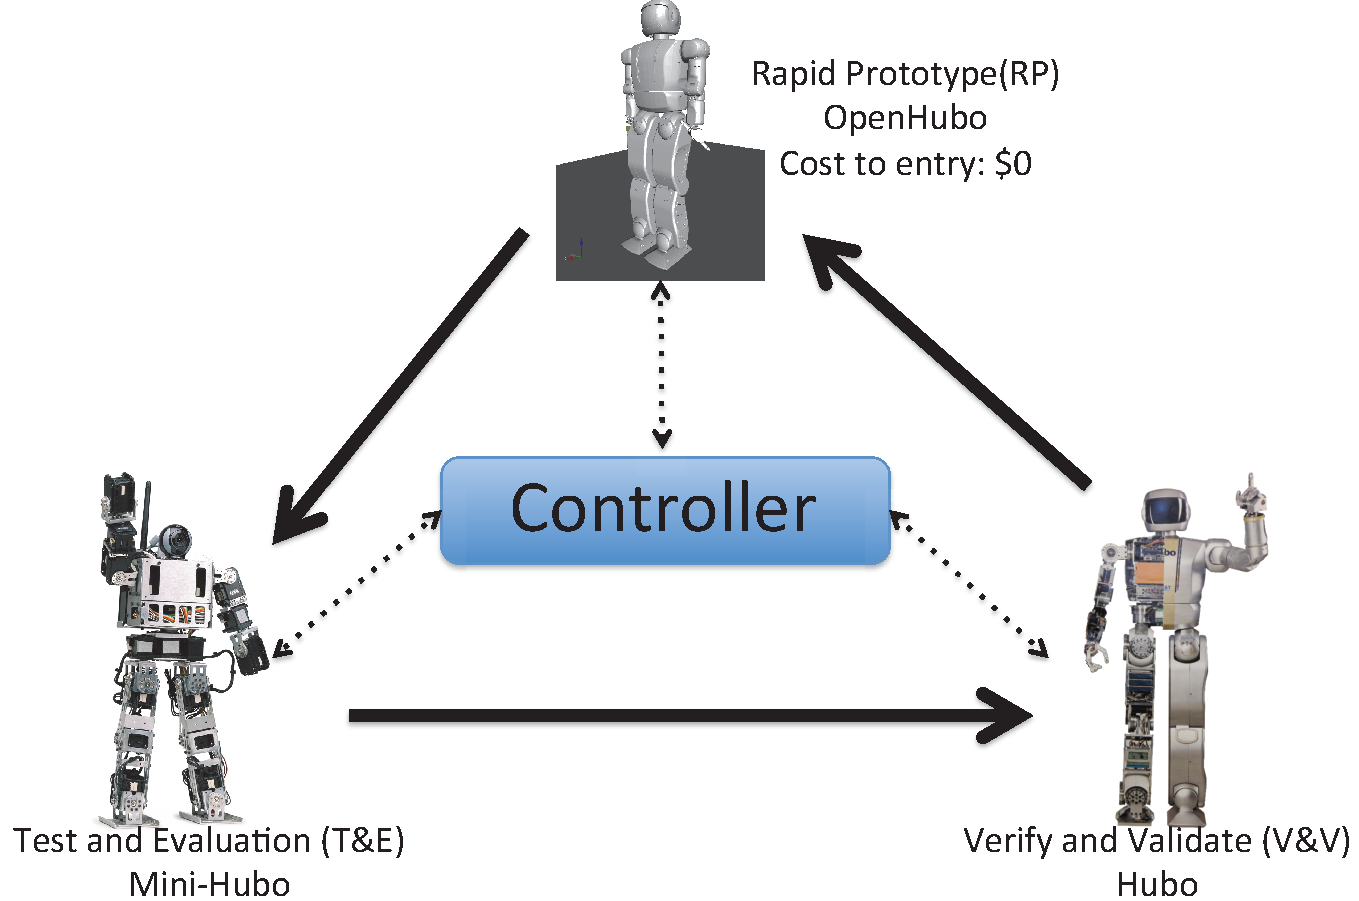
\includegraphics[angle=90, width=0.8\columnwidth]{./pix/threeTier.pdf}
  \caption{Three tier infrastructure. Tier 1: Rapid Prototype (RP) using OpenHubo. Tier 2: Test and Evaluation (T\&E) using Mini-Hubo.  Tier 3: Verify and Validate (V\&V) using Hubo.}
  \label{fig:threeTier}
\end{figure}




	\section{Challenges}\label{sec:challenges}
		\input{background/challenges.tex}


%%------ Inspiration -------%%	
	\section{Inspiration: DARPA Robotics Challenge}\label{sec:drc}
    	In July 2012 DARPA released a solicitation for proposals to compeat in the DARPA Robotics Challenge (DRC).
The DRC is a challenge that is in direct response to the Tsuanmi in Psuicima in 2010 (check this).
The challenge is to have a robot be able to use human tools, human vehicles and proform human tasks in an un-structured un modified human enviroment.
We applied for the grant.
In October 2012 we received word that we are a Track-A team for the DRC.
This means that we are competing agains NASA, Raythion, CMU and a team from Japan.
One of the keys to our team is our collaberation.
We are partnered with WPI, Georgia Tech, University of Delleware, Swarthmore, Purdue, Ohio State (check that) and RAINBOW (a company that rose from the Hubo Lab at Korea Advanced Institute of Science and Technology (KAIST)).
Each partner would be responsiable with one event.
We will then combine our efforts into one master controller that is cabiable of doing all the given tasks.
Having a multi-process system that also gives us the ability for our partners to share their controllers without having to intergrate their code.  
Controllers run indipendently.
	
    	%% Add DRC Pix	

%%------ Virtical Leap  -------%%	
    	\section{Controbutions and Vertical Leap}
		The primary contributions and vertical leap to the field is the creation of a \textit{unified algorithmic framework for high degree of freedom complex systems and humanoid robots}.
The resulting framework allows seamless integration of:
\begin{itemize}
\item Controllers running at different loop rates
\item Runs on multiple robots with no modification
\item Runs on simulated robots with no modification 
\item Inherent structure makes it more robust
\item Written in C for controller programing language interdependence (use C bindings in desired language)
\end{itemize}
The unified frame work Hubo-Ach is an Open-Source BSD licensed software allowing for open use.

The contributions of Hubo-Ach have been independently verified by external parties\cite{tepraDoor2013,tepraCut2013}.
Is has been validated by multiple IEEE publications\cite{lofaroTePRA2013HuboAch,lofaroTePRA2013Valve}, in review for a publication in the IEEE Robotics and Automation Society Magazine (RAM)\cite{lofaroRAM2013} and has been the top featured video on the IEEE Spectrum \textit{Video Friday} article on December 14$^{th}$, 2012\cite{videoFriday}.

		%% Works with other stuff

   	\section{Increasing Degrees of Freedom}\label{sec:numdof}
		Degree of freedom (DOF) is the number of independent parameters that can be varied in a mechanical system.
Simply put the DOF of a robot is the number independent joints the robot contains.
In modern robot implementation each joint is controlled by an actuator.
Each actuator is controlled by the controller.
The more DOF the more complex the controller.

In the early 1930s simple two DOF robots were used by the soviets as explosive devices\cite{robotTelitankSpringer2013military}.
These robots were remote control and had no mind of their own.
In 1948 William Grey Walter created the first autonomous robots \textit{Tortoise Elmer} and \textit{Elise}\cite{robotElmer}.
Each of these simple two DOF robots were programmed in hardware to go towards a light source.  
This was referred to as BEAM Robot (Biology, Electronics, Aesthetics, and Mechanics) because of how the hardware configuration mimicked the electrical connections in an animals brain.
In later years robots were being programmed in software to help create the first industrial robot UNIMATE which was a 6 DOF arm created by General Motors in 1954\cite{handbookOnRobotics2008springer}.  
Lunokhod 2, a soviet lunar rover which landed on the moon in 1973, was equipped with a laser ranging system and a TV camera.
It contained 11 DOF and had automated systems onboard, however it was primarily a remote controlled vehicle.
By 1986 Rodney Brooks, co-founder and CTO of iRobot Corp., created Allen, a 18 DOF humanoid robot.
The complexity and number of DOF keeps on increasing.
By 1997 Honda completed the 28 DOF P3, a early version of what will become ASIMO \cite{robotsAsimo1041641}.
Today with the presents of HUBO, ASMO and HRP-4C it is common place for a robot to contain upwards of 40 DOF.
A study done on 180 robots from the early 20$^{th}$ century to the present projects that by the year 2020 it will be as common to have a 70 DOF robot as it is to have a 40 DOF robot in 2013, see Fig.~\ref{fig:numOfRobots}. 
\textit{The trend of increasing DOF in robots makes creating a control structure for these systems timely.}


These high DOF robots require complex control systems and strategies.



Creating controllers for these high degree of freedom complex systems is essential for development of the next generation of robots.
Due to the inherent complexity and often high expense of these systems, controllers must be able to be tested and verified.



\begin{figure}[thpb]
  \centering
      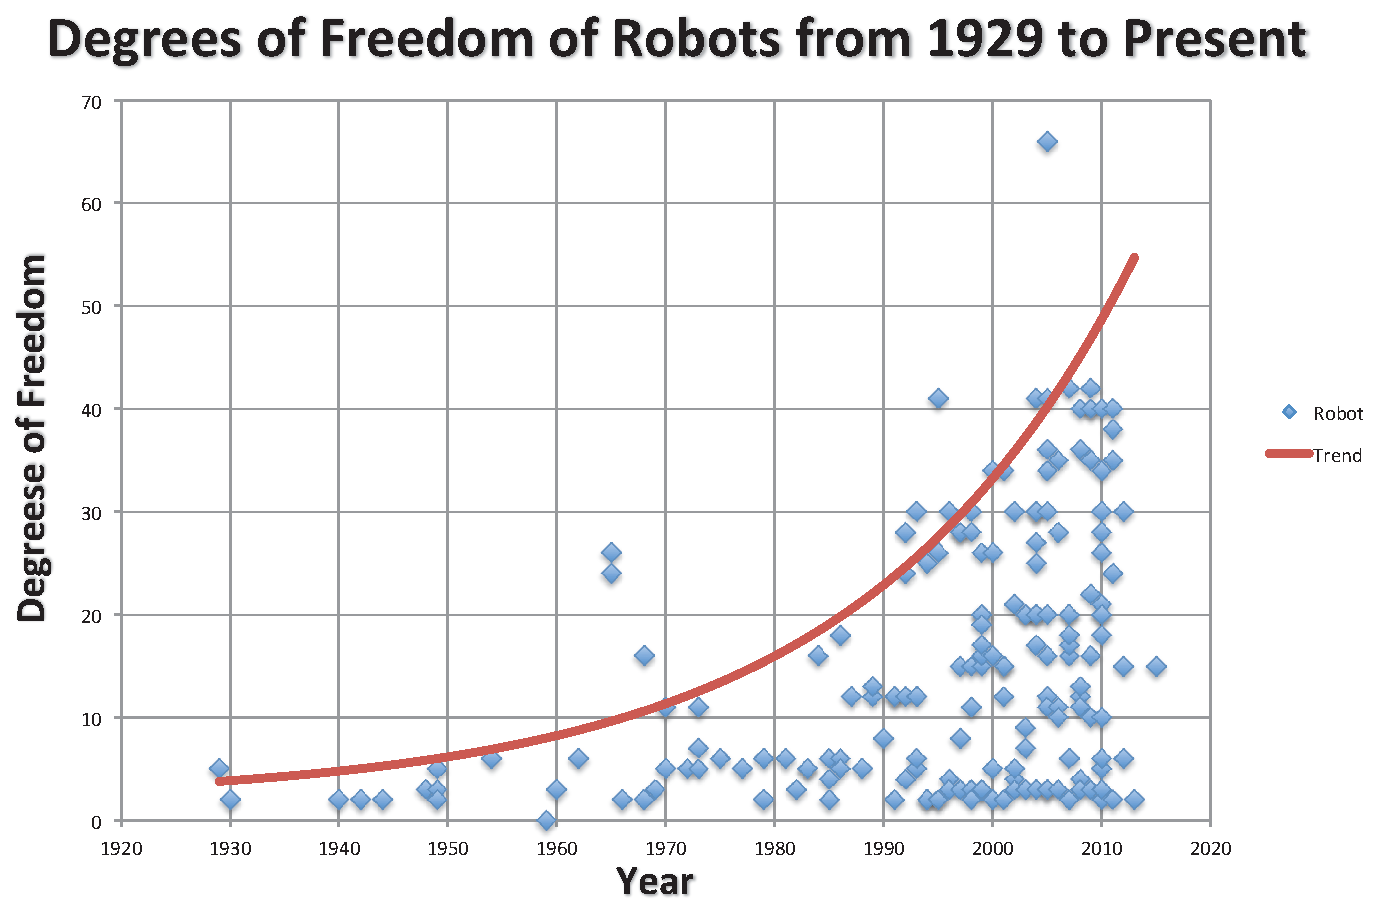
\includegraphics[width=0.8\columnwidth]{./pix/robotsDOF.pdf}
\caption{Number of degrees of freedom for robots form 1929 to the present.}
\label{fig:numOfRobots}
\end{figure}





			
			
			
			
			

	

 %Introduction
	\chapter{Background and Results from Preliminary Experiments}\label{sec:background}

This section gives brief background and results from preliminary experiments of the methods used to complete the Hubo-Ach system.
The motivation and timeline of experiments is given in Section~\ref{sec:roadmap}.

Section~\ref{sec:back:hubo-ach} describes why inter-process communication (IPC) is used for the Hubo-Ach control system and a brief background of different IPC methods.
Section~\ref{sec:hubo-ach} give this background in greater detail.


%%------ Path To Ph.D. -------%%	
	\section{Motivation}\label{sec:roadmap}	
		This section provides context to the origin of the idea of a unified algorithmic framework for complex systems.

%%%%%%% Put what I wrote here
\begin{figure}[thpb]
  \centering
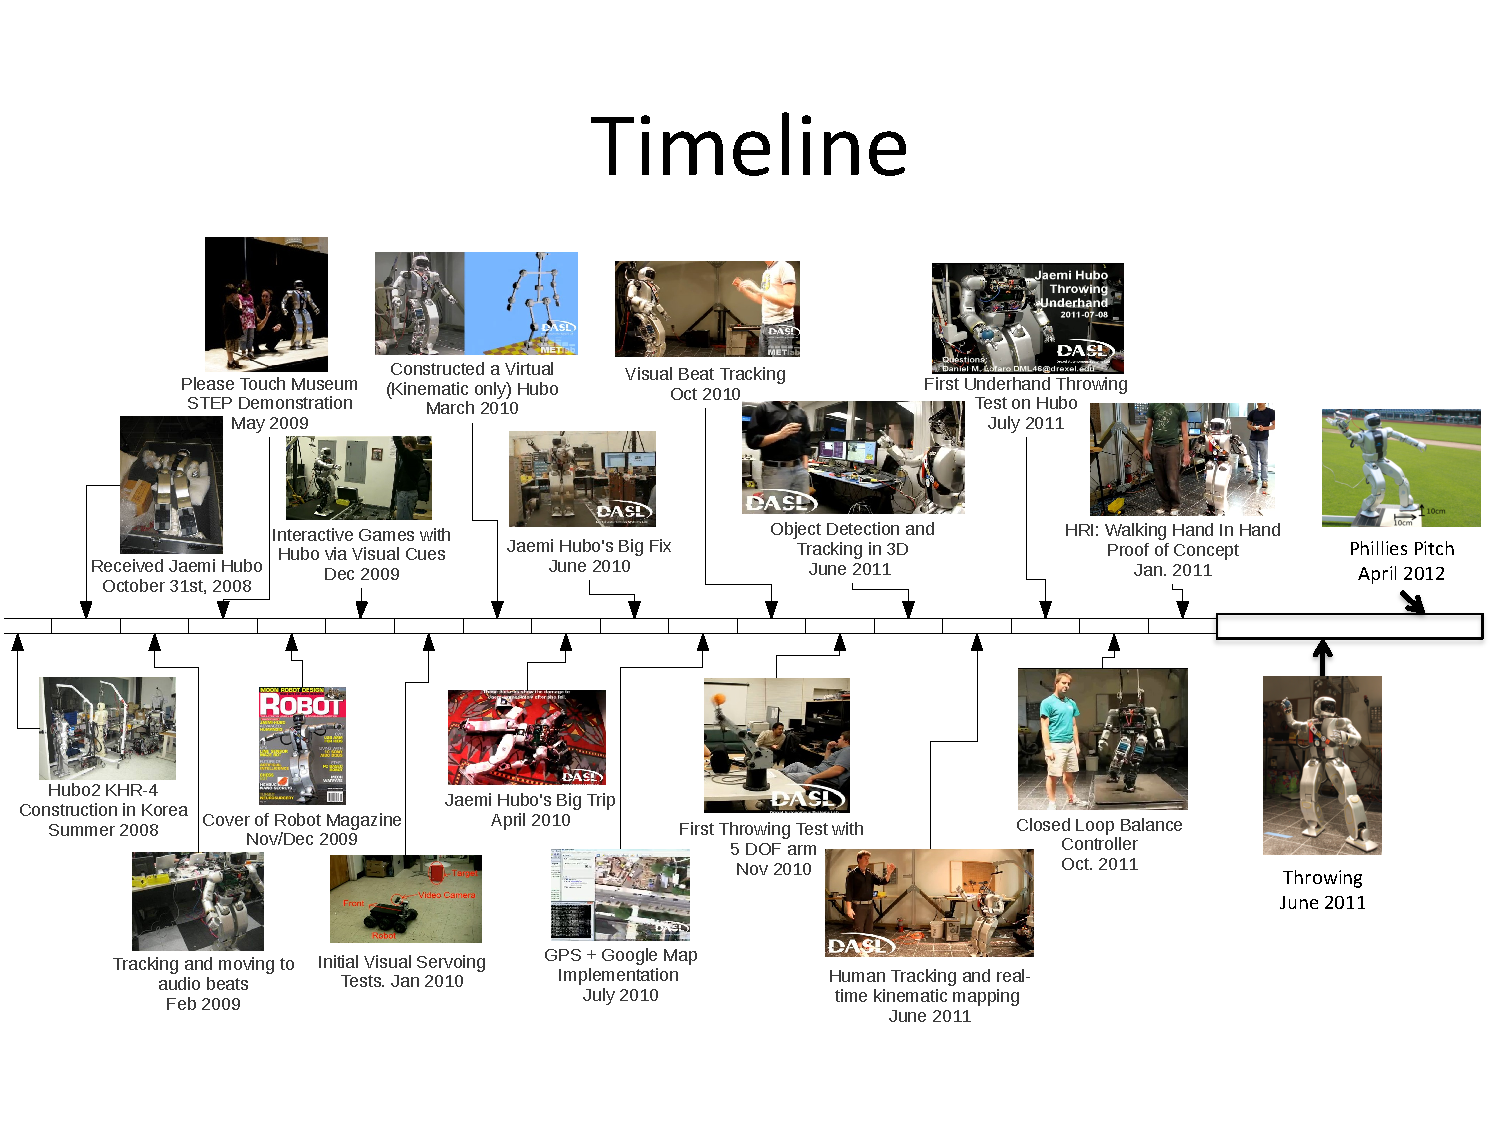
\includegraphics[angle=90, width=0.9\columnwidth]{./pix/Timeline.pdf}
  \caption{Timeline of Daniel M. Lofaro's research from 2008 to 2012}
  \label{fig:timeline}
\end{figure}

\subsection{Human Robot Interaction}
The initial goal was to have a humanoid robot become an interactive musical participant with humans.
This spawned the creation of a visual method of tracking the beat in the absence of auditory cues\cite{5686847}.
This came from a modification of a method of allowing children to play interactive games with humanoid robots\cite{lofaroGamesRobot}.
The resulting method was effective, but to increase the accuracy it was required to combine a pre-existing auditory beat tracker with the visual system.
This calumniated with a multi process system that combine the auditory and visual beat trackers\cite{lofaroIASTED2011,6094987,lofaroEURASIP2011}.
A human comparison was completed and found that this combined method was as accurate at detecting the beat in music as average humans.

\subsubsection{Results from preliminary experiments}
When collaborating with other to create a complex robot control systems integrating controllers is difficult because of the use of:
\begin{itemize}
\item different loop rates causing synchronization issues
\item different programming languages making using the same libraries a challenge
\end{itemize}

It was found that it is best to keep each working systems \textit{independent} allowing them to run at their native rate and on their native platforms\cite{ach}.



\subsection{High Degree of Freedom Kinematic Planning}
The next challenge was to perform kinematic planning for end effector velocity control. 
This resulted in the development of a method that is able to solve inverse kinematics (IK) for high degree of freedom (DOF) systems where there is no closed-form solution as well as create collision free trajectories for high DOF robots\cite{6385987}.
This is described in detail in Section~\ref{sec:srm} and \ref{sec:baseball}.
This culminated in the verification and validation of the system by an experiment where Hubo full-size humanoid robot throw the first pitch at a Major League Baseball (MLB) game\cite{lofaroHumanoids2012,6462956}.

\subsubsection{Results from preliminary experiments}
As best practice when controllers and planners are implemented it is important that low-level controllers such as balance and obstacle avoidance run at all times\cite{lofaroRAM2013}. 
Non-priority controllers such as throwing trajectory planning can run in the background in a separate process.
Keeping the processes separate allowed the system to be more resistant to lag and crashes of one or more of the controllers.
This brought validation to the overarching plan for the unified algorithmic framework for complex systems and humanoid robots.




\subsection{Lessons Learned}

At this point creating these experiment it was required to \textit{hacked} together pre-existing systems that allowed the robot to do the task.
This is the point where it was realized that a \textit{unified algorithmic framework for complex systems and humanoid robots} was required for further development in the field.
Key lessons learned from these experiments were:
\begin{itemize}
\item Must inherently decouple controllers loop rates and phases
\item Must allow for collaborators not have to \textit{inject} their code into existing source.
\item Must work with multiple robots for testing, evaluation, validation, and verification.
\end{itemize}

\noindent This is where Hubo-Ach was born.
The idea was to create a multi process architecture for humanoid control using state of the art high-speed low-latency Inter-Process Communication (IPC) techniques\cite{lofaroRAM2013}.
This is different from traditional IPC techniques because of the lack of head of line (HOL) blocking and focus on low-latency.
Section~\ref{sec:ipc} gives further details and comparisons of different IPCs.


The need for this unified framework was amplified when the Hubo was chosen to be the primary platform for the DRC-Hubo\footnote{DRC-Hubo: http://www.drc-hubo.com/} Track-A team.
Since its initial conception Hubo-Ach has become a fully functional system used in active research by multiple universities including MIT, WPI, Purdue, Ohio State, Swarthmore College, Georgia Tech, and Drexel University\cite{lofaroTePRA2013HuboAch,lofaroTePRA2013Valve}.
This research also acts as a key source of verification and validation of the system.


		

		\section{Control System Structures}\label{sec:back:struct}
			The traditional single loop control structure that is used in robot control software such as Orocos\cite{orocos-gadeyne-ijrr2005}, Microsoft Robot Studio\cite{microsoftRobot4437755}, RobotC\cite{robotc}, and LabVIEW\cite{labview} are not suited for high DOF robots.
Due to the nature of these highly redundant complex electrical mechanical system it is common to desire multiple different controllers running in tandem.  
Different controllers are needed when the system is in different states or doing different tasks or performing multiple tasks at the same time.
Combining these controllers is a problem in complex system.
This problem is hard when each controller has different loop rates that are not even multiples of on another, timing requirements (asynchronous vs. synchronous).

Multi-threaded approaches using shared memory allow for compatibility of multiple loop rates such as in Lee et. al.\cite{multi-thread-robot-5602743} with multi-threaded controllers on their humanoids, Rai et. al.\cite{multi-thread-snake-1541141} with multi-threaded controllers on their snake robots and Zheng et. al.\cite{multi-thread-5524083} with multi-threaded controllers on their under water robots.
The multi-threaded approach still has an inherent flaw.
If the parent or one of the other controller threads crashes it is difficult or impossible to restart the controller and still have access the the shared memory.

By using a multi process approach allows controllers to fault and restart with minimal effect on the other controllers.
Typical ways of communicating between different processes is via UDP or TCP/IP such as OpenHRP\cite{openHRP} with their server based control platform for the HRP humanoid robot; Aramaki et. al.\cite{multiPC-arch-1185243} and Lofaro et. al.\cite{lofaroIASTED2011} with their multi-computer based control methods and the popular Robot Operating System (ROS)\cite{ros} by Willow Garage.

Communicating via TCP/IP sockets, such as in OpenHRP and ROS, guarantee that the data is received but it does not guarantee a arrival time.
This means if the checksum fails the message will be sent again increasing the latency of the message.
This does not work well if a real-time control loop is required.
Using UDP does not resend if the checksum fails.
This keeps the latency low and is better for real-time applications such as in the work of Lofaro.
Both UDP and TCP/IP require that the buffer is read before new data is read.
This means that you must read the older data before newer data.
This is called head of line blocking or HOL\cite{ach}.

Newer state information is preferred by robots that work in the physical world over older data.  
Thus it is desired that HOL is eliminated.
This can be done with some forms of inter-process communication (IPC).

OpenHRP and Webots\cite{Webots} are two of the very short list of systems that have simulators that use the same controller as the hardware platforms.
However at this time to the best of our knowledge there is no system that:
\begin{itemize}
\item uses the same controller with the software and hardware systems
\item is inhreently robust by using a multi-process approach
\item uses low-latency methods for controller communications 
\end{itemize}





	
		\section{Multi-Process and Interprocess Comunication}\label{sec:back:hubo-ach}
	    		
This section gives a quick background to why inter-process communication (IPC) is used for the Hubo-Ach control system and a brief background of different IPC methods.
Section~\ref{sec:hubo-ach} give this background in greater detail.

The idea for a Control Architecture for High DOF robots stems from a gap in physical implementation of control algorithms for robot hardware.
The simplest approach to developing robot software is to integrate all functionality in one program.  
This functionality includes the following controllers:
\begin{multicols}{2}
\begin{itemize}
\item Hardware Control
\item Perception
\item Planning
\item Kinematics
\item etc.
\end{itemize}
\end{multicols}

If all of this functionality is in one process then it has the benefit of freedom of inter process communication latency.
However being in one process also means that if one of the controllers lags or faults it cause the entire controller to lag or fault.
This is of great concern if a non-priority controller such as vision processing faults causing a priority controller such as a balance controller, to fail.
This will cause the robot to fall.
How is this fixed?
One solution and my proposed solution is to use multiple processes and IPC methods.
Inter-process communication is a method of exchanging data between multiple processes.
Typical POSIX methods give you the \textbf{oldest} information first and have locks on the memory when processes are writing to it.
An overview of these mechanisms are given in \cite{stevens2005advanced}.

Robots work in the physical world. 
More recent information is more important to it then older.
In most cases it is acceptable to know the most recent data and never read any of the older data.
This would happen if your sensors update at a faster rate then that of the robot.
Typically robot actuators have a bandwidth much much lower then that of a modern computer.
If sensor information is shared using traditional shared memory over POSIX methods the controller would have to read the older information before it reaches the information it is most interested in, the newest data.
This is known effect but new concern for robot controllers called head of line blocking\cite{ach}.

It is desired to make a multi-process controller that can share data between multiple processes with low-latency and no head of line blocking.
There are a few IPCs that offer no head of line blocking and low-latency.  
A description of each IPC type is in Section~\ref{sec:hubo-ach}.
Table~\ref{table:ipc} shows a full comparison of the different IPC types.
%After much research (inserte examples here) it was found that the Ach IPC wuld best fit my needs.

My thesis Hubo-Ach is a multi-process control system that uses IPC methods to communicate between processes.
Section~\ref{sec:hubo-ach} describes Hubo-Ach in detail.



	    		
	    		
	%%------ About Hubo -------%%
	\section{Platforms}\label{sec:robots}
	This section describes the different platforms that are focused on in this document.
		\subsection{Hubo2 Plus}\label{sec:hubo}
			%\subsubsection{Hubo2 Plus}
The Hubo2+ is a $1.3\meter$ (4' 3'') tall, 42 $kg$ (93 $lb$) full-size
humanoid robot.  The Hubo series was designed and constructed by the
Korean Advanced Institute of Science and Technology (KAIST) and
spinoff Rainbow Inc. \cite{hubofirst}.  It has 38 degree of freedom:
six per arm and leg, five per hand, three in the neck, and one in the
waist.  Sensors include three-axis force-torque sensors in the wrists
and ankles, accelerometers in the feet, and an inertial measurement
unit (IMU).  The sensors and embedded motor controllers are connected
via a Controller Area Network to a pair of Intel Atom PC104+ PCs
running a GNU/Linux distribution.



% The reference commands for
% all of the joints are sent from the primary control computer (x86) to
% the individual motor controllers via two Controller Area Network (CAN)
% buses.  This is the same communications bus found in most modern motor
% vehicles.  There are currently eight Hubo's functioning in the United
% States as of December 2012.  Four reside at Drexel University and one
% at Georgia Tech, Purdue, Ohio State and MIT.  Jaemi Hubo is the oldest
% of the Hubos in America and has been at the Drexel Autonomous Systems
% Lab\footnote{Drexel Autonomous Systems Lab:
%   http://dasl.mem.drexel.edu/} (DASL) since 2008 \cite{jaemiHuboSRM}.
% Fig.~\ref{fig:hubo} shows the major dimensions of Hubo.

% \begin{figure}[thpb]
%   \centering
% \includegraphics[width=1.0\columnwidth]{./pix/huboSkel.pdf}
%   \caption{Hubo2 Plus platform: 38 DOF, 130 $cm$ tall full-size humanoid robot weighing 37 $kg$.}
%   \label{fig:hubo}
% \end{figure}

% All joints of the major joints are high gain PID position
% controlled with the exception of the fingers.  The fingers are
% open-loop PWM controlled.
% The sensing capability consists of a three
% axis force-torque (FT) sensor on each leg between the end of the ankle
% and the foot as well as between the arm where it connects to the hand.
% Additionally it has an inertial measurement unit (IMU) at the center
% of mass and accelerometers on each foot.

%%% Local Variables:
%%% mode: latex
%%% TeX-master: "ach"
%%% End:

		\subsection{Mini-Hubo}\label{sec:mini-hubo}
			Mini-Hubo\cite{threeTier} is a miniture version of the Hubo platform discribe in Section~\ref{sec:hubo}.
It is used as the Test and Evaluation (T\&E) stage of the three tier infrastructure discribed in Section~\ref{sec:threeTier}.
Mini-Hubo is kinematically scaled to the Hubo platform.
The atrobutes of the Mini-Hubo system are in Table~\ref{table:huboMiniSensors}.
The robot is shown in Fig.~\ref{fig:mini-hubo}


\begin{table}
\centering
\caption{Mini-Hubo Platform Specifications}
\begin{tabular}{| l || l |}
\hline
Height      		& $46~cm$			\\
\hline
Weight			& $2.9~kg$			\\
\hline
DOF			& 22				\\
\hline
Joint Control Type	& PID Position			\\
\hline
Computer		& $1.6~Ghz$ Atom		\\
			& $2~Gb$ DDR2 RAM		\\
\hline
Operating System	& Debian Linux			\\
\hline
Battery			& $14.8V$ $3.2~Ah$ $30C$ LiPo	\\
\hline
Sensors			& 2x 3 Axis Force Torque	\\
\hline
Vision			& Monocular			\\
			& RGBD				\\
\hline
\end{tabular}
\label{table:huboMiniSensors}
\end{table}





\begin{figure}[thpb]
  \centering
\includegraphics[width=0.37\columnwidth]{./pix/mini-hubo.jpg}
  \caption{Mini-Hubo platform: 22 DOF, 46 $cm$ tall miniture-size humanoid robot weighing 2.9 $kg$.}
  \label{fig:mini-hubo}
\end{figure}

		\subsection{OpenHubo}\label{sec:openhubo}
			OpenHubo\cite{dlofaro-srm} is an open-source kinematic and dynamic simulator for the the Hubo2 and Hubo2+ series robots.
It was developed by the Drexel Autonomous Systems Lab and runs using the open-source robot simulation environment OpenRAVE\cite{diankovThesis}.
Fig.~\ref{fig:openhubo1} shows the OpenHubo model.
Table~\ref{table:huboOpenSensors} shows the spesifications of OpenHubo.


\begin{figure}[thpb]
  \centering
      \includegraphics[width=0.4\columnwidth]{./pix/hBody.png}\includegraphics[width=0.4\columnwidth]{./pix/hCol.png}
      
\caption{OpenHubo model of the Hubo2 humanoid robot developed by the Drexel Autonomous Systems Lab and runs using the open-source robot simulation environment OpenRAVE\cite{diankovThesis}.}
\label{fig:openhubo1}
\end{figure}


\begin{table}
\centering
\caption{OpenHubo Platform Specifications}
\begin{tabular}{| l || l |}
\hline
Dynamics      		& Yes (ODE)			\\
\hline
Kinematic		& Yes				\\
\hline
DOF			& 40				\\
\hline
Joint Control Type	& PID Position			\\
\hline
Computer		& $1.6~Ghz$ Atom		\\
			& $2~Gb$ DDR2 RAM		\\
\hline
Enviroment		& OpenRAVE\cite{diankovThesis}	\\

\hline
Sensors			& 1x 4 Axis IMU			\\
			& 4x 3 Axis Force Torque	\\
\hline
\hline
\end{tabular}
\label{table:huboOpenSensors}
\end{table}

		

	\chapter{Methodology}
%% Intro to methodology


%% --------- Balancing ----------
\section{Balancing}\label{sec:sec:balance}
	\input{pitch/balancing.tex}




%% ------------ Thorwing ---------------
\section{Throwing}\label{sec:baseball}
	Since 2005  
Creating controllers for high degree of freedom complex systems is essential for development of the next generation of robots.
Due to the inherent complexity and often high expense of the system, controllers must be able to be tested.



It is common place for a complex electrical mechanical system to have multiple different controllers running in tandem.  
Different controllers are needed when the system is in different states or doing different tasks.
Combining these controllers is a problem in complex system.
This problem is hard when each controller has different frequencies, timing requirements (asyncronous vs. syncronous), latency restrictions, newest state data ie smore important then older state data and most basic of all languages the controller is written in.
This is especially true for complete and complex autonomous systems.
I define a complete and complex autonomous system as an electro mechanical mechanism with high degree of freedom (DOF) that is capable of making its own decisions through the use of sensor data processed by its artificial intelligence (AI).
The combination of high DOF and the requirement for autonomy makes the work space broad and controllers complex.
The overarching question becomes; What is the control system structure for a complete and complex autonomous systems with high DOF, a multitude of sensors, AI performing high-level and low-level tasks all while keeping a stable system structure conducive to collaborative work?
Current methods of solving the problem of controller synchrony and latest state data is to keep your critical control elements in the primary control loop.
Inter-process communication (IPC) and/or network sockets to communicate between the high level and low level processes even if written in different languages.
The majority of IPC have the problem of \textit{head of line} blocking (HOL) which means you must read the older data in a buffer before you read the newest data.
In the computer science field this is not a problem because all data being intact is typically desired.  
In the field of robotics and control the most recent state data is more important to a real-time control system to act on.
This thesis shows that by expanding on the idea of multi-process controllers connected to high-speed low-latency IPC you can create a \textit{robot layer} on a computer platform that will allow low-level controllers to run in separate processes while still allowing them access to the most recent data as the priority.
The new technical idea is the \textit{robot layer}, a control layer that allows external processes to run like normal and not deal with the specifics of the given robot system.
The robot system can be replaced by a simulated system without any of the processes needing to be modified or even know of the change.
This allows more mature controllers to be easily interfaced with this system without modifying control rates or timing.
This \textit{robot layer} must be:
\begin{itemize}
\item Have a IPC latency much less then that of the robot's inherent sampling period $t_{ipc}<<T_{r}$
\item Allow for command rates much slower then the inherent sampling period $T_{slow}>>T_{r}$
\item Allow for command rates much faster then the inherent sampling period $T_{fast}<<T_{r}$
\item Allow for arbitrary command rates.
\item Allow for real-time and non-real-time controllers to command actuators
\item Allow for all processes to have access to the newest data first
\item Allow for no more then one rt time step delay between command and robot actuator retrieval
\item Commanded such that it is for an arbitrary robotic actuator.
\item Triggering for process synchronization
\item Triggering for simulator synchronization and holding
\end{itemize}
We can succeed now not only because the bleeding edge technology allows for the fast enough communication between processes with access to the latest data.

Results are measured quantitatively and qualitatively.
Data showing proper loop rates, timings, controller implementation, simulation connections etc. show the viability of the system.
User survey shows methodology is sound, useful, and practical.





My Thesis shows is that a multi-process control structure coupled with the proper timing mechanisms is conducive to answering these questions.
It is shown with physical experiments and the creation of Hubo-Ach\cite{lofaroRAM2013}; a fully functional Sim-Time and Real-Time control system for complete and complex autonomous systems.

Through experimentation I prove my control system is a viable way of controlling complete and complex autonomous system and still be conducive to collaborative work.  
A road map of how my research has taken me to my thesis is shown in Section~\ref{sec:roadmap}.
As proof of viability I show the basic structure of my system \textit{Hubo-Ach} in Section~\ref{sec:hubo-ach}.  
I give step by step examples in Section~\ref{sec:simpleExamples}.
Section~\ref{sec:simulator} shows how we can move from real-time to using a simulated version of the platform in simulation time without having to change the controller.
Section~\ref{sec:task} describes the experiment which consists of making the robot preform an advanced task that pulls together visual, kinematic, path planning and other controllers together using this one system.
The techniques used stem from my contributions in Section~\ref{sec:contributions}.
Section~\ref{sec:results} shows the results of the experiment thus show the viability of the system.
Lastly Section~\ref{sec:conclusion} discusses the results of the work and the future of this system.

Before I continue it is important to note that my work has already been validated by my pears because:
\begin{itemize}
\item It was chosen to be the primary control system for the DARPA Robotics Challenge Track-A Team DRC-Hubo, Section~\ref{sec:drc}.
\item It is being used in the NSF-MIRR project\footnote{NSF-MIRR: Major Research Infrastructure Recovery and Reinvestment (MIRR) \#CNS-0960061 sponsored by the the U.S. National Science Foundation (NSF)}.
\item It is currently being used by MIT, WPI, Purdue, Ohio State, Swarthmore College, Georgia Tech, and Drexel University.
\end{itemize}

For the remainder of this document the complete and complex autonomous systems that I will be referring to are robots.
The majority of examples given will be in reference to humanoid robotics and the Hubo2+ (KHR-4+) platform.
The Hubo platform is described in Section~\ref{sec:hubo}.





	
	\subsection{Throwing Using Sparse Reachable Map}\label{sec:sec:srm}
		\input{pitch/srm.tex}

	\subsection{Human to Humanoid Kinematic Mapping}\label{sec:sec:mocap}
		\input{pitch/mocap.tex}

	\subsection{Key-Frame Motion}\label{sec:sec:keyframe}
		\input{pitch/keyframe.tex}

%% --------- SRM - make sure they know this is what I did
\section{Sparse Reachable Map Velocity Space Inverse Kinematics}\label{sec:srm}
		%\begin{center}
\large\bf{Abstract:}
\end{center}
\normalsize

\bf{
\noindent The degrees of freedom (DOF) of robots and complex systems have been increasing increasing exponentially since the early 20th century.
Today it is common place for complex control systems to have 40 DOF. 
This number is projected to be 70 DOF by the year 2020.
Robots with high DOF allows for complex tasks such as tool manipulation, greater human-robot interaction and agile full-body locomotion.
More DOF require greater attention to local communication delays, bandwidth, system configuration and stability.
In addition different tasks being performed by separate parts of the robot in tandem bring on greater issues including controller timing and priorities.
The increase in DOF on single system requires that the traditional methods of controller design be re-examined.

\noindent This dissertation describes a Unified Algorithmic Framework for High Degree of Freedom Complex Systems and Humanoid Robots that allows a user to develop controllers using a three tier infrastructure.
The Unified Algorithmic Framework called Hubo-Ach is a multi-process based system that allows for robust multi-rate simultaneous control and seamless implementation between virtual, miniature, and full-size robots with no modification.
The three tier infrastructure provides different levels of cost to entry and testing.
Examples of this field tested framework functioning on simulated, miniature, and full-size high DOF robots is given as well as validation by external researchers.
}




		%Since 2005  
Creating controllers for high degree of freedom complex systems is essential for development of the next generation of robots.
Due to the inherent complexity and often high expense of the system, controllers must be able to be tested.



It is common place for a complex electrical mechanical system to have multiple different controllers running in tandem.  
Different controllers are needed when the system is in different states or doing different tasks.
Combining these controllers is a problem in complex system.
This problem is hard when each controller has different frequencies, timing requirements (asyncronous vs. syncronous), latency restrictions, newest state data ie smore important then older state data and most basic of all languages the controller is written in.
This is especially true for complete and complex autonomous systems.
I define a complete and complex autonomous system as an electro mechanical mechanism with high degree of freedom (DOF) that is capable of making its own decisions through the use of sensor data processed by its artificial intelligence (AI).
The combination of high DOF and the requirement for autonomy makes the work space broad and controllers complex.
The overarching question becomes; What is the control system structure for a complete and complex autonomous systems with high DOF, a multitude of sensors, AI performing high-level and low-level tasks all while keeping a stable system structure conducive to collaborative work?
Current methods of solving the problem of controller synchrony and latest state data is to keep your critical control elements in the primary control loop.
Inter-process communication (IPC) and/or network sockets to communicate between the high level and low level processes even if written in different languages.
The majority of IPC have the problem of \textit{head of line} blocking (HOL) which means you must read the older data in a buffer before you read the newest data.
In the computer science field this is not a problem because all data being intact is typically desired.  
In the field of robotics and control the most recent state data is more important to a real-time control system to act on.
This thesis shows that by expanding on the idea of multi-process controllers connected to high-speed low-latency IPC you can create a \textit{robot layer} on a computer platform that will allow low-level controllers to run in separate processes while still allowing them access to the most recent data as the priority.
The new technical idea is the \textit{robot layer}, a control layer that allows external processes to run like normal and not deal with the specifics of the given robot system.
The robot system can be replaced by a simulated system without any of the processes needing to be modified or even know of the change.
This allows more mature controllers to be easily interfaced with this system without modifying control rates or timing.
This \textit{robot layer} must be:
\begin{itemize}
\item Have a IPC latency much less then that of the robot's inherent sampling period $t_{ipc}<<T_{r}$
\item Allow for command rates much slower then the inherent sampling period $T_{slow}>>T_{r}$
\item Allow for command rates much faster then the inherent sampling period $T_{fast}<<T_{r}$
\item Allow for arbitrary command rates.
\item Allow for real-time and non-real-time controllers to command actuators
\item Allow for all processes to have access to the newest data first
\item Allow for no more then one rt time step delay between command and robot actuator retrieval
\item Commanded such that it is for an arbitrary robotic actuator.
\item Triggering for process synchronization
\item Triggering for simulator synchronization and holding
\end{itemize}
We can succeed now not only because the bleeding edge technology allows for the fast enough communication between processes with access to the latest data.

Results are measured quantitatively and qualitatively.
Data showing proper loop rates, timings, controller implementation, simulation connections etc. show the viability of the system.
User survey shows methodology is sound, useful, and practical.





My Thesis shows is that a multi-process control structure coupled with the proper timing mechanisms is conducive to answering these questions.
It is shown with physical experiments and the creation of Hubo-Ach\cite{lofaroRAM2013}; a fully functional Sim-Time and Real-Time control system for complete and complex autonomous systems.

Through experimentation I prove my control system is a viable way of controlling complete and complex autonomous system and still be conducive to collaborative work.  
A road map of how my research has taken me to my thesis is shown in Section~\ref{sec:roadmap}.
As proof of viability I show the basic structure of my system \textit{Hubo-Ach} in Section~\ref{sec:hubo-ach}.  
I give step by step examples in Section~\ref{sec:simpleExamples}.
Section~\ref{sec:simulator} shows how we can move from real-time to using a simulated version of the platform in simulation time without having to change the controller.
Section~\ref{sec:task} describes the experiment which consists of making the robot preform an advanced task that pulls together visual, kinematic, path planning and other controllers together using this one system.
The techniques used stem from my contributions in Section~\ref{sec:contributions}.
Section~\ref{sec:results} shows the results of the experiment thus show the viability of the system.
Lastly Section~\ref{sec:conclusion} discusses the results of the work and the future of this system.

Before I continue it is important to note that my work has already been validated by my pears because:
\begin{itemize}
\item It was chosen to be the primary control system for the DARPA Robotics Challenge Track-A Team DRC-Hubo, Section~\ref{sec:drc}.
\item It is being used in the NSF-MIRR project\footnote{NSF-MIRR: Major Research Infrastructure Recovery and Reinvestment (MIRR) \#CNS-0960061 sponsored by the the U.S. National Science Foundation (NSF)}.
\item It is currently being used by MIT, WPI, Purdue, Ohio State, Swarthmore College, Georgia Tech, and Drexel University.
\end{itemize}

For the remainder of this document the complete and complex autonomous systems that I will be referring to are robots.
The majority of examples given will be in reference to humanoid robotics and the Hubo2+ (KHR-4+) platform.
The Hubo platform is described in Section~\ref{sec:hubo}.





		\input{srm/priorwork.tex}
		\section{Methodology}\label{sec:methodology}
\input{pitch/balancing.tex}
\input{pitch/mocap.tex}
\input{pitch/srm.tex}
\input{pitch/keyframe.tex}

		%% split trapozoidal motion profile into another section example


\section{Final Design}\label{sec:finalDesign}
	\input{pitch/finalDesign.tex}

\section{Conclusion}\label{sec:throw:conclusion}
	Throwing using the key-frame based method was the most reliable and successful.  
	The system was open-loop in respect to the location where it would throw the ball.
	This is why it over threw the ball during the real pitch, see Fig.~\ref{fig:hubo-throw-test}.
	The lessons learned when performing the throwing task is that
	\begin{enumerate}
		\item A unified algorithmic framework is needed for three tier testing
		\item Using such a framework the loop has to be closed on the ball's final location
		\item System for having a stable landing when taking a step
	\end{enumerate}

	Section~\ref{sec:hubo-ach} describes the unified framework that answer \#1 above.
	As stated before throwing is a full body locomotive task. 
	Section~\ref{sec:visuralServoing} closes the loop using visual methods.
	This shows how the unified algorithmic architecture can be used for visual servoing a full body locomotive tasks.
	This visual servoing example answer \#2 above.
	The use of active damping as seen in Section~\ref{sec:activedamping} allows the robot to land on the ground.
	This answers \#3 above.



		

	%\chapter{Control System for Complete Complex Autonomous Systems: Hubo-Ach}\label{sec:hubo-ach}
%\chapter{Thesis: Hubo-Ach - A Control System for Complete Complex Autonomous Systems}\label{sec:hubo-ach}
\chapter{Thesis: Control System for Complete Complex Autonomous Systems}\label{sec:hubo-ach}

%% Hubo-Ach Inspiration
\section{Overview}

%% Hubo-Ach explanation
%% workign wth ros and other software that exists, why in C


\input{hubo-ach/hubo-ach-intro.tex}
\section{Inter Process Comunication Comparision}
	POSIX provides three main types of IPC: streams, datagrams and shared memory.  
A review of each is made before making a choice for desired message passing skeam.

\noindent \textbf{Streams:}\\
The IPC type \textit{stream} includes pipes, FIFOs, stream sockets, and TCP sockets.
All stream basted methods suffer from head of line (HOL) blocking which means older data \textbf{must} be read before newer data.
%In addition all streaming methods are exposed to file abstraction (read/write byte sequence).
For robotic applications we must be able to access the newest data imediately and read older data if needed.
This is a different paradime then typical streaming application because robots are real-time sensitive meaning the newest information holds more value to the overall system than the older data.

\noindent \textbf{Datagrams:}\\
POSIX \textit{datagrams} come in two major flavors, \textit{datagram sockets} and \textit{POSIX message queues}.
Datagram sockets are less likely to block the sender then streams.
The most important reason why datagrams are \textbf{not} a good solution for my application is that newer messages are lost if the buffer is filled.
Newer data is more important than older data in my control system thus this is not a viable option.

POSIX message queues are simular to datagrams sockets with the addition of message priorities.
Unlike datagram sockets if the buffer fills the POSIX message queues will block.
This will cause the application to stop processing until it is able to read/flush the old messages.
Thus simular to other methods mentioned this also suffers from HOL.

\noindent \textbf{Shared Memory:}\\
POSIX shared memory is very fast and allows access to the latest data by simply writing over a variable.
Though I have been advicating that the newest information is the most important, old information can not be discarded.
If using POSIX shared memory there is no way of recovering older data that might have been missed by a controller.

What is needed is a method of sharing data that is \textit{non-blocking} and as \textit{low-latancy} like shared memory, but still holds older data and uses an asyncronous IO scheme.
The asyncronous IO scheme is required so the controller is not locked to a set rate by the data transactionn method.
N. Dantam et. al.\cite{ach} shows that Asynchronous IO (AIO) might be approperiate for this application however the implimentaiton under Linux is not as mature as I require.
In addition N. Dantam shows that other IPC mechanism using select/poll/epoll/kqueue are widely used network server and help midigate but not totally removed the issue of HOL.
The primary problem being that that thought the sender will not block the reader must stil read the oldest data first.
The question now is what IPC mechanism will be suitable for my control system.

Upon investigation three major mechanisms are avaliable; Robot Operating System (ROS)\cite{ros}, Message Passing Interface (MPI)\cite{Gropp:1999:UMP:330577} and Ach\cite{ach}.
Though ROS is ubicuitious in the robotics and automation field the inherent latency and the non real-time (RT) guarantee due to the use of TCP/IP it is not a good choice.
MPI is ubiquitous in the high-proformance computing field.  It has full non-blocking capiabilities and is geared towards maximizing message throughput for networked clusters\cite{ach}.
Table~\ref{table:ipc} shows a comparision of a wide range of IPC methods.
A focus on reducing latency is not given.
Ach is a newer 

\begin{table}
\caption{Robot control system comparison}
\begin{tabular}{l || c | c | c | c | c | c}
\hline
System                          & Open        & POSIX           & Non          & Real      & Low         & Light \\
                                &      Source &       Complaint &     Blocking &      Time &     Latency & Weight\\
\hline
\hline
ROS                             & yes         & yes             & no           & no        & no          & no \\
\hline
Orocos Real-Time                & yes         & yes             & no           & yes       & yes         & no \\
                 Toolkit        &             &                 &              &           &             &    \\
\hline

Robotics Technology             & yes         & yes             & no           & yes       & yes         & no \\
                    Middleware  &             &                 &              &           &             &    \\
\hline
Microsoft Robotics              & no          & no              & no           & yes       & yes         & no \\
                   Studio       &             &                 &              &           &             &    \\
\hline
Aware2.0                        & no          & yes             & no           & yes       & yes         & yes \\
\hline
Hubo-Ach                        & yes         & yes             & yes          & yes       & yes         & yes \\



\hline
\end{tabular}
\label{table:robotOS}
\end{table}


\begin{table}
\caption{Inter Process Comunication Method Comparison}
\small
\begin{tabular}{l || c | c | c | c | c | c | c}
\hline
Inter-                          & Open        & POSIX           & Non          & Multiple    & Low         & Light   & Access \\
Process                         &      Source &       Complaint &     Blocking & Senders     &     Latency & Weight  & Old   \\
Comunication                    &             &                 &              & and         &             &         & Data          \\
Method                          &             &                 &              & Receivers   &             &         &           \\
\hline
\hline
Streams                         & yes         & yes             & no           & yes       & no          & yes     & yes \\
\hline
Datagram                        & yes         & yes             & no           & yes       & no          & yes     & yes \\
Sockets                         &             &                 &              &           &             &         &     \\
\hline

POSIX                           & yes         & yes             & no           & yes       & no          & yes     & yes\\
Message                         &             &                 &              &           &             &         &     \\
Queues                          &             &                 &              &           &             &         &     \\
\hline
Shared                          & yes         & yes             & yes          & yes       & yes         & yes     & no \\
Memory                          &             &                 &              &           &             &         &     \\

\hline
AIO                             & yes         & yes             & yes          & yes       & yes         & yes     & yes \\
\hline
CORBA                           & yes         & yes             & yes          & no        & yes         & yes     & yes \\
\hline
ROS                             & yes         & yes             & no           & yes       & no          & no      & no \\
\hline
Data                            & yes         & yes             & yes          & yes       & yes         & yes     & yes\\
Distribution                    &             &                 &              &           &             &         &     \\
Service                         &             &                 &              &           &             &         &     \\
\hline
Ach                             & yes         & yes             & yes          & yes       & yes         & yes     & yes\\


\hline
\end{tabular}
\label{table:ipc}
\normalsize
\end{table}


\section{Timing}
	\begin{figure}
\centering

\begin{tikzpicture}[->,>=stealth',shorten >=1pt,auto,node distance=5cm,
  thick,main node/.style={fill=white!20,draw,font=\sffamily\footnotesize\bfseries}]

  
  \node[main node] (latesRef) [ text width=2.0cm, minimum height=1.5cm, align=center]   {Reference\\(Latest)};
  \node[main node] (ctrl)     [left=0.8cm of latesRef,minimum height=2.5cm, align=center]                           {Controller};
  \node[main node] (getRef)   [right=1.5cm of latesRef, text width=3.0cm, minimum height=1.1cm, align=center]      {Get Reference};
 

 % \node[main node] (fromsim)     [above=1.0cm of getRef, text width=3.0cm, minimum height=1.1cm, align=center]    {From Simulator\\ Hold (sim mode)};
 % \node[main node] (sim)         [above=1.0cm of fromsim, text width=3.0cm, minimum height=1.1cm, align=center]    {Simulator \\Trigger\\ (sim mode)};

 \node[main node, draw=white] (haname2)   [above=0.2cm of getRef, align=center]   {};

  \node[main node] (dodebug)     [below=1.0cm of getRef, text width=3.0cm, minimum height=1.1cm, align=center]    {User Commands\\ (debug)};
  \node[main node] (tosim)       [below=1.0cm of dodebug, text width=3.0cm, minimum height=1.1cm, align=center]    {To Simulator\\ Trigger};
  \node[main node] (filter)      [below=1.0cm of tosim, text width=3.0cm, minimum height=1.1cm, align=center]     {Filter};
  \node[main node] (setRef)      [below=1.0cm of filter, text width=3.0cm, minimum height=1.1cm, align=center]    {Set Reference};
  \node[main node] (reqSens)     [below=1.0cm of setRef, text width=3.0cm, minimum height=1.1cm, align=center]    {Request Sensors};
  \node[main node] (getSens)     [below=1.0cm of reqSens, text width=3.0cm, minimum height=1.1cm, align=center]   {Get Sensors};
  \node[main node] (canWait)     [below=1.0cm of getSens, text width=3.0cm, minimum height=1.1cm, align=center]   {Wait on CAN};
  \node[main node] (putState)    [below=1.0cm of canWait, text width=3.0cm, minimum height=1.1cm, align=center]   {Put State};
  \node[main node] (rthold)      [left=0.5cm of getSens, minimum height=1.1cm, align=center]   {Real-Time\\Hold};



  \node[main node] (latestState) [left=1.5cm of putState, text width=2.0cm, minimum height=1.1cm, align=center, yshift=-1.0cm]   {State\\(Latest)};
  \node[main node, draw=white] (haname)   [right=3.0cm of putState, align=center]   {};

  \node[main node] (robot)    [right=4.8cm of getSens, minimum height=5.5cm, align=center]    {Robot};
  

%H_ref.ref[jnt] = deg;
%H_ref.mode[jnt] = HUBO_REF_MODE_ENC_FILTER;

  \path[->, dashed,every node/.style={font=\sffamily\small}]
    (ctrl) edge node [above] {} (latesRef);

%  \path[->, every node/.style={font=\sffamily\small}]
%    (fromsim) edge node [right] {$t_0=0.011~ms$} (getRef);
%\draw[->] ([xshift=-1.2 cm]fromsim.south)  to [out=-90,in=90] node [right] {$t_0=0.011~ms$} ([xshift=-1.2 cm]getRef.north)  ;
%\draw[->] ([xshift=-1.2 cm]getRef.south)   to [out=-90,in=90] node [right] {$t_1=0.011~ms$} ([xshift=-1.2 cm]tosim.north)  ;
%\draw[->] ([xshift=-1.2 cm]tosim.south)   to [out=-90,in=90] node [right] {$t_2=0.011~ms$} ([xshift=-1.2 cm]filter.north)  ;
%\draw[->] ([xshift=-1.2 cm]filter.south)   to [out=-90,in=90] node [right] {$t_3=???~ms$} ([xshift=-1.2 cm]setRef.north)  ;
%\draw[->] ([xshift=-1.2 cm]setRef.south)   to [out=-90,in=90] node [right] {$t_4=???~ms$} ([xshift=-1.2 cm]reqSens.north)  ;
%\draw[->] ([xshift=-1.2 cm]reqSens.south)   to [out=-90,in=90] node [right] {$t_5=???~ms$} ([xshift=-1.2 cm]getSens.north)  ;
%\draw[->] ([xshift=-1.2 cm]getSens.south)   to [out=-90,in=90] node [right] {$t_6=0.011~ms$} ([xshift=-1.2 cm]putState.north)  ;
%\draw[->] ([xshift=0.0 cm]putState.west)   to [out=180,in=-90] node [below, yshift=-0.5cm, xshift=-0.2cm] {$t_7=0.011~ms$} ([xshift=0.0 cm]rthold.south)  ;


\draw[->] ([xshift=0.0cm]latesRef.east)  to [out=0,in=-180]  node [right]  {} ([xshift=0.0cm]getRef.west)  ;
%\draw[->] ([xshift=0.0cm]fromsim.south)  to [out=-90,in=90]  node [right]  {} ([xshift=0.0cm]getRef.north)  ;
\draw[->] ([xshift=0.0cm]getRef.south)   to [out=-90,in=90]  node [right]  {} ([xshift=0.0cm]dodebug.north)  ;
\draw[->] ([xshift=0.0cm]dodebug.south)  to [out=-90,in=90]  node [right]  {} ([xshift=0.0cm]tosim.north)  ;
\draw[->] ([xshift=0.0cm]tosim.south)    to [out=-90,in=90]  node [right]  {} ([xshift=0.0cm]filter.north)  ;
\draw[->] ([xshift=0.0cm]filter.south)   to [out=-90,in=90]  node [right]  {} ([xshift=0.0cm]setRef.north)  ;
\draw[->] ([xshift=0.0cm]setRef.south)   to [out=-90,in=90]  node [right]  {} ([xshift=0.0cm]reqSens.north)  ;
\draw[->] ([xshift=0.0cm]reqSens.south)  to [out=-90,in=90]  node [right]  {} ([xshift=0.0cm]getSens.north)  ;
\draw[->] ([xshift=0.0cm]getSens.south)  to [out=-90,in=90]  node [right]  {} ([xshift=0.0cm]canWait.north)  ;
\draw[->] ([xshift=0.0cm]canWait.south)  to [out=-90,in=90]  node [right]  {} ([xshift=0.0cm]putState.north)  ;
\draw[->] ([xshift=0.0 cm]putState.west) to [out=180,in=-90] node [below, yshift=-0.5cm, xshift=-0.2cm] {} ([xshift=0.0 cm]rthold.south)  ;
\draw[->] ([xshift=0.0 cm]rthold.north)  to [out=90,in=-120] node [left, yshift=-1.0cm, xshift=-0.8cm, rotate=90] {} ([xshift=0.0 cm]getRef.west)  ;
\draw[->] ([xshift=0.0cm]putState.south) to [out=-90,in=0]   node [right]  {} ([xshift=0.0cm]latestState.east)  ;




%\draw[->] ([yshift=0.75cm]fromsim.east)  to [out=-30,in=30] node [right] {$t_0=0.014~ms$} ([yshift=-0.75cm]fromsim.east)  ;
\draw[->] ([yshift=0.75cm]getRef.east)  to [out=-30,in=30] node [right] {$t_0=0.010~ms$} ([yshift=-0.75cm]getRef.east)  ;
\draw[->] ([yshift=0.75cm]dodebug.east)  to [out=-30,in=30] node [right] {$t_1=0.011~ms$} ([yshift=-0.75cm]dodebug.east)  ;
\draw[->] ([yshift=0.75cm]tosim.east)  to [out=-30,in=30] node [right] {$t_2=0.014~ms$} ([yshift=-0.75cm]tosim.east)  ;
\draw[->] ([yshift=0.75cm]filter.east)  to [out=-30,in=30] node [right] {$t_3=0.008~ms$} ([yshift=-0.75cm]filter.east)  ;
\draw[->] ([yshift=0.75cm]setRef.east)  to [out=-30,in=30] node [right] {$t_4=0.152~ms$} ([yshift=-0.75cm]setRef.east)  ;
\draw[->] ([yshift=0.75cm]reqSens.east)  to [out=-47,in=47] node [right] {$t_5=1.365~ms$} ([yshift=-0.75cm]getSens.east)  ;
\draw[->] ([yshift=0.75cm]canWait.east)  to [out=-30,in=30] node [right,align=center] {$t_6=3.000~ms$\\(hard timeout)} ([yshift=-0.75cm]canWait.east)  ;
%\draw[->] ([yshift=0.75cm]reqSens.east)  to [out=-30,in=30] node [right] {$t_5=???~ms$} ([yshift=-0.75cm]reqSens.east)  ;
%\draw[->] ([yshift=0.75cm]getSens.east)  to [out=-30,in=30] node [right] {$t_6=???~ms$} ([yshift=-0.75cm]getSens.east)  ;
\draw[->] ([yshift=0.75cm]putState.east)  to [out=-30,in=30] node [right] {$t_7=0.092~ms$} ([yshift=-0.75cm]putState.east)  ;
\draw[->] ([yshift=-0.75cm]rthold.west)  to [out=120,in=-120] node [above, yshift=1.5cm, xshift=0.3cm, rotate=90] {$\displaystyle t_{hold}=T-\sum_{i=0}^{8} t_i=0.348~ms$} ([yshift=0.75cm]rthold.west)  ;

\draw[->, dashed] ([xshift=0.0cm]latestState.west)   to [out=120,in=-90] node [right] {} ([xshift=0.0cm]ctrl.south)  ;
%\draw[->, dashed] ([xshift=0.0cm]sim.south)   to [out=-90,in=90] node [right] {} ([xshift=0.0cm]fromsim.north)  ;

\node[fit=(getRef)(putState)(rthold)(haname)(latestState)(haname2), draw,label={south:Hubo-Ach}] (hubo-ach) [minimum width=4.5cm] {};




\draw[->,loosely dotted] ([xshift=0.75cm]reqSens.south)  to [out=-30,in=-180] node [above] {} ([yshift=0.75cm]robot.west)  ;
\draw[<-,loosely dotted] ([xshift=0.0cm]getSens.east)  to [out=0,in=-180] node [above, xshift=1.7cm] {CAN} ([yshift=0.0cm]robot.west)  ;
\draw[<-,loosely dotted] ([xshift=0.75cm]canWait.north)  to [out=30,in=-180] node [above] {} ([yshift=-0.75cm]robot.west)  ;




%  \path[->,every node/.style={font=\sffamily\small}]
%    (ik) edge node [above] {$\overline{\theta_d}$} (filter);

% \draw[->] ([xshift=-0.5 cm]filter.south)  -- node [left] {$\overline{\theta_r}$} ([xshift=-0.5 cm]hubo-ach.north)  ;
% \draw[->] ([xshift=0.5 cm]hubo-ach.north) -- node [left] {$\overline{\theta_a}$} ([xshift=0.5 cm]filter.south)  ;

% \path[<->,dashed, every node/.style={font=\sffamily\small}]
%    (hubo) edge node [above] {CAN} (hubo-ach);


\end{tikzpicture}
\caption{Timing diagram of Hubo-Ach.  All times $t_*$ denote measured times each block takes to complete.  Tests were done on a 1.6Ghz Atom D525 Dual Core with 1GB DDR3 800Mhz memory running Ubuntu 12.04 LTS linux kernel 3.2.0-29 on a Hubo2+ utilizing a CAN bus running at 1Mbps baud.  Average CPU usage is 7.6\% using a total of 4Mb or memory.}
\label{fig:hubo-ach-timing}
\end{figure}




	\chapter{Experiment}
%% Explain the tasks

%%%\section{System setup}
%%%State diagram of plan
%%%\begin{itemize}
%%%\item Find the valve - sensing
%%%\item Move to the valve - close loop on sensing
%%%\item Grab the valve
%%%\item Jump on the valve
%%%\end{itemize}


%%%\section{Task}\label{sec:task}
%%%Turning a valve with whole body (more of a lever)
%%%\begin{itemize}
%%%\item Find the valve - sensing
%%%\item Move to the valve - close loop on sensing
%%%\item Grab the valve
%%%\item Jump on the valve
%%%\end{itemize}

%%%Controllers
%%%\begin{itemize}
%%%\item Walking
%%%\item Balance
%%%\item Complience
%%%\item IK
%%%\item Visual Servoing
%%%\end{itemize}




\section{Balance}
%% Once foot example
%% maybe 2 foot example

\section{Simulator}\label{sec:simulator}
	The simulator used for Hubo-Ach is the OpenHubo.
OpenHubo is an open-source kinematic and dynamic simulator for the the Hubo2 and Hubo2+ series robots.
It was developed by the Drexel Autonomous Systems Lab and runs using the open-source robot simulation environment OpenRAVE\cite{diankovThesis}.
Fig.~\ref{fig:openhubbo} shows the OpenHubo shell model and collision model.

\begin{figure}[thpb]
  \centering
      \includegraphics[width=0.4\columnwidth]{./pix/hBody.png}\includegraphics[width=0.4\columnwidth]{./pix/hCol.png}
      
\caption{OpenHubo model of the Hubo2 humanoid robot developed by the Drexel Autonomous Systems Lab and runs using the open-source robot simulation environment OpenRAVE\cite{diankovThesis}.  (Left) Shell Model - High polygon count.  (Right) Collision model - Made with primitives.}
\label{fig:openhubbo}
\end{figure}

The masses and lengths are of the OpenHubo model are all based off of the CAD model.
The shell model includes an external skin based off of the CAD model of the Hubo's shell.
This model is high polygon count and thus tends to require more processing time to detect collisions.
The collision model is constructed out of primitives in order to decrease the complexity of the model and decrease required processing time.
The collision model is a representation of the shell model. 
It does not precisely fit the contours but through experimentation and use has been calibrated to be a good representation of the Hubo's outer shell.

Fig~\ref{fig:openhubosim} shows the diagram of how the OpenHubo simulator is connected to Hubo-Ach.  
No changes to previous controllers are required for them to work with the simulator.
Just as before the desired reference $\theta_d$ being filtered before applied to Hubo via Hubo-Ach.  
$\theta_d$ is sent through a filter that reduces the \textit{jerk} on the actuator then the new reference $\theta_r$ is set on the \textbf{FeedForward} channel, Hubo-Ach reads it then commands Hubo at the rising edge of the next cycle.  
At this point the \textit{to simulator} trigger, $\Gamma_{ts}$, is set high and the OpenHubo simulator reads $\theta_c$.
The simulator waits until Hubo-Ach is ready until it starts its next set of cycles.
The reference is set within OpenHubo and solved with a simulation period of $T_{sim}$.
The simulation period $T_{sim}$ must be an integer deviser of the robot real-time period $T_r$.
In this case

\begin{equation}
T_r=0.005~s
\end{equation}

\begin{equation}
T_{sim} = \frac{T_r}{n}
\end{equation}


Once the simulator has gone through $n$ cycles the current state, $H_{state}$ is placed on the Hubo-Ach \textbf{FeedForward} channel and the ready trigger $\Gamma_{fs}$ is raised.  
Hubo-Ach is waiting for the rising edge of the \textit{from simulator} trigger, $\Gamma_{fs}$, to continue on to the next cycle.

\begin{figure}
\centering

\begin{tikzpicture}[->,>=stealth',shorten >=1pt,auto,node distance=5cm,
  thick,main node/.style={fill=white!20,draw,font=\sffamily\Large\bfseries}]


  \node[main node] (ctrl) {Controller};
  \node[main node] (filter) [right=1.5cm of ctrl] {Filter};
  \node[main node] (hubo-ach) [below=1.0cm of filter] {Hubo-Ach};
  
  \node[main node,font=\small] (hold1) [right=1.5cm of hubo-ach, yshift=0.5cm] {hold};
  \node[main node,font=\small] (hold2) [right=1.5cm of hubo-ach, yshift=-0.5cm] {hold};

  \node[main node] (hubo) [right=1.5cm of hold1, yshift=-0.5cm] {OpenHubo};




%  \path[->, every node/.style={font=\sffamily\small}]
%    (hubo-ach) edge node [above] {$\theta_c$} (hubo);

\draw[->] ([yshift=0.2 cm]hubo-ach.east)  to [out=0,in=-180] node [below] {$\theta_c$} ([yshift=-0.0 cm]hold1.west)  ;
\draw[->] ([yshift=0.0 cm]hold1.east)  to [out=0,in=-180] node [below] {$\theta_c$} ([yshift=0.2 cm]hubo.west)  ;
\draw[-*] ([xshift=1.0 cm]hubo-ach.north)  to [out=60,in=120] node [above] {$\Gamma_{ts}$} ([yshift=-0.05 cm]hold1.north)  ;



\draw[->] ([yshift=0.0 cm]hold2.west)  to [out=180,in=0] node [below] {$H_{state}$} ([yshift=-0.2 cm]hubo-ach.east)  ;
\draw[->] ([yshift=-0.2 cm]hubo.west)  to [out=180,in=0] node [below right] {$H_{state}$} ([yshift=0.0 cm]hold2.east)  ;
\draw[-*] ([xshift=0.0 cm]hubo.south)  to [out=-120,in=-60] node [above] {$\Gamma_{fs}$} ([yshift=0.05 cm]hold2.south)  ;

\draw[->] ([yshift=-0.0 cm]hubo-ach.west)  to [out=180,in=-90] node [below left] {$H_{state}$} ([yshift=0.0 cm]ctrl.south)  ;



%\draw[->] ([yshift=-0.2 cm]hubo.west)  -- node [below] {$H_{state}$} ([yshift=-0.2 cm]hubo-ach.east)  ;
%\draw[->] ([yshift=-0.0 cm]hubo.south)  to [out=-120,in=-60] node [below] {$\Gamma_{fs}$} ([yshift=-0.0 cm]hubo-ach.south)  ;



  \path[->,every node/.style={font=\sffamily\small}]
    (ctrl) edge node [above] {$\theta_d$} (filter);

 \draw[->] ([xshift=-0.5 cm]filter.south)  -- node [left] {$\theta_r$} ([xshift=-0.5 cm]hubo-ach.north)  ;
 \draw[->] ([xshift=0.5 cm]hubo-ach.north) -- node [left] {$\theta_a$} ([xshift=0.5 cm]filter.south)  ;


\end{tikzpicture}
\caption{Diagram of how the OpenHubo simulator is connected to Hubo-Ach.  No changes to previous controllers are required for them to work with the simulator.  Just as before the desired reference $\theta_d$ being filtered before applied to Hubo via Hubo-Ach.  $\theta_d$ is sent through a filter that reduces the \textit{jerk} on the actuator then the new reference $\theta_r$ is set on the \textbf{FeedForward} channel, Hubo-Ach reads it then commands Hubo at the rising edge of the next cycle.  At this point $\Gamma_{ts}$ is set high and the OpenHubo simulator reads $\theta_c$.  The reference is set within OpenHubo and solved with a simulation period of $T_{sim}$.  Once The state, $H_{state}$ has been determined it is placed on the Hubo-Ach \textbf{FeedForward} channel and the ready trigger $\Gamma_{fs}$ is raised.  Hubo-Ach is waiting for the rising edge of $\Gamma_{fs}$ to continue on to the next cycle.}
\label{fig:openhubosim}
\end{figure}




The external controllers do not know weather Hubo-Ach is running in \textit{simulation} or \textit{real-time} mode.  
In order to ensure a Hubo-Ach controller stays what ever timing method is being used the controller can do any of the following:

\begin{itemize}
\item Wait for the $\Gamma_{fs}$ trigger
\item Wait for a new $H_P{state}$ to be updated
\item Watch the time listed within $H_{state}$
\end{itemize}

If the given task does not require physics or feedback from $H_{state}$ then you can run in \textit{no physics} mode.
\textit{No physics} mode only gives collisions, joint angles and ideal feedback from the sensors.
In addition \textit{no physics} is capable of running much faster then real-time if needed.



\begin{table}
\centering
\caption{OpenHubo simulator sim-time and real-time comparison chart.  Shows the maximum percent real-time the OpenHubo simulator is capable of preforming at where 100\% is real-time.  All tests were preformed on an Intel i7 running at 2.8Ghz with 18Gb of RAM.}
\begin{tabular}{| l || c | c |}
\hline
Mode               & Timing                & Maximum Percent Real-Time (\%) \\
\hline
\hline
Physics            & Sim-Time              & 37\%   \\
\hline
No Physics         & Real-Time or Sim-Time & 362\%  \\
\hline
\end{tabular}\label{table:simtime}
\end{table}


Fig.~\ref{fig:visualservoing} shows the capability of Hubo-Ach to run in both sim-time and real-time modes.  
This is the same statically stable trajectory as seen in Fig.~\ref{fig:staticwalking}


\begin{figure}[thpb]
  \centering
      \includegraphics[width=0.93\columnwidth]{./pix/tmp.png}
      \includegraphics{./qrcode/qrcode-simtimewalking.png}\\
      Video: http://danlofaro.com/phd/simtimewalking/
\caption{OpenHubo walking using Hubo-Ach in Sim-Time mode with ODE physics.}
\label{fig:visualservoing}
\end{figure}


	%% show balance in simulator too








%% Advanced Examples: Maybe add the title :advanced examples or somethign like that			
\section{Visual Serving Example}
This section uses visual feedback using an RGB-D (Red Green Blue - Depth) camera and the 6-DOF IK example from Section~\ref{sec:6dofik}.
	\subsection{Tracking Using Vision}
		This section discribes how to intergrate color tracking the 6-DOF IK controller derived in Section~\ref{sec:6dofik}.
\begin{figure}
\centering

\begin{tikzpicture}[->,>=stealth',shorten >=1pt,auto,node distance=5cm,
  thick,main node/.style={fill=white!20,draw,font=\sffamily\small\bfseries}]

  \node[main node] (vis) [text width=3cm] {Object Tracking};
  \node[main node] (ref) [below=1.0cm of vis] {Desired Position};
  \node[main node] (ik) [right=2.0cm of ref] {6-DOF IK};
  \node[main node] (filter) [right=2.0cm of ik] {Filter};
  \node[main node] (hubo-ach) [below=1.0cm of filter] {Hubo-Ach};
  \node[main node] (hubo) [right=2.0cm of hubo-ach] {Hubo};



  \path[->, every node/.style={font=\sffamily\small}]
    (ref) edge node [above] {$(x,y,z)$} (ik)
    (ref) edge node [below] {$(\alpha,\beta,\gamma)$} (ik);
%  \path[->, every node/.style={font=\sffamily\small}]
%    (ref) edge node [below] {$(\alpha,\beta,\gamma)$} (ik);

 
  \path[->,every node/.style={font=\sffamily\small}]
    (vis) edge node [right] {$(x,y,z)$} (ref);

  \path[->,every node/.style={font=\sffamily\small}]
    (ik) edge node [above] {$\overline{\theta_d}$} (filter);

 \draw[->] ([xshift=-0.5 cm]filter.south)  -- node [left] {$\overline{\theta_r}$} ([xshift=-0.5 cm]hubo-ach.north)  ;
 \draw[->] ([xshift=0.5 cm]hubo-ach.north) -- node [left] {$\overline{\theta_a}$} ([xshift=0.5 cm]filter.south)  ;

 \path[<->,dashed, every node/.style={font=\sffamily\small}]
    (hubo) edge node [above] {CAN} (hubo-ach);

%  \path[->,every node/.style={font=\sffamily\small}]
%    (hubo-ach) edge node [left] {$\theta_r$} (filter);

%  \path[->,every node/.style={font=\sffamily\small}]
%    (filter) edge node [right] {$\theta_a$} (hubo-ach);




% look into this and add z^-1

%\path [every node/.style={draw,minimum width=3cm, minimum height=5cm]}]
%  node (a) at (0,0) {}
%  [xshift=7cm]
%  node (b) at (0,0) {}
%  [xshift=7cm]
%  node (c) at (0,0) {};

%\begin{scope}[->,>=latex]
%    \foreach \i in {-2,...,2}{% 
%      \draw[->] ([yshift=\i * 0.8 cm]a.east) -- ([yshift=\i * 0.8 cm]b.west) ;}

%    \foreach \i in {1,2}{% 
%      \draw[->] ([yshift=\i * 0.8 cm]a.east) to [out=50,in=130] ([yshift=\i * 0.8 cm]c.west) ;} 

%    \foreach \i in {-1,-2}{% 
%      \draw[->] ([yshift=\i * 0.8 cm]a.east) to [out=-50,in=-130] ([yshift=\i * 0.8 cm]c.west) ;}
%\end{scope}


\end{tikzpicture}
\caption{The $(x,y,z)$ work space position of the obje}
\label{fig:hubo-ach-feedforwardFilterFeedBack}
\end{figure}



Using a simple HSV (Hue Saturation Value) 



\begin{figure}[thpb]
  \centering
      \includegraphics[width=0.69\columnwidth]{./examples/pix/hsv.png}
      \includegraphics[width=0.3\columnwidth]{./qrcode/qrcode-hsvtrackingexample.png}\\
      Video: http://danlofaro.com/phd/tracking/\#HsvTracking
\caption{3D Object tracking using HSV color matching and an RGB-D camera to gain depth information.}
\label{fig:visualservoing}
\end{figure}

		



\section{Walking}
	%% Sim walking too
	This section shows examples of how Hubo-Ach was used for stable walking.
Examples are given using:
\begin{itemize}
\item Hubo2+ (Physical Robot)
\item OpenHubo (Simulator)
\item RobotSim Hubo (Simulator)
\end{itemize}

section~\ref{sec:WalkingPatternGeneration} shows how the open-loop walking trajectory is created.

Section~\ref{sec:OpenHuboWalking} shows how the open loop walking trajectory is run in sim-time on OpenHubo using Hubo-Ach.
Section~\ref{sec:RobotSimWalking} shows how the open loop walking trajectory is run in sim-time on RobotSim using Hubo-Ach.
Section~\ref{sec:HuboWalking} shows the same walking trajectory running on the real Hubo hardware in real-time using Hubo-Ach.
It also shows the difference between running in sim-time and real-time.
Section~\ref{sec:dynamicWalking} shows the result of a five day \textit{hack-a-thon} using Hubo-Ach to add dynamic walking capability.





%% ---------------- Walking Pattern Generation ------------------------
\subsection{Walking Pattern Generation}\label{sec:WalkingPatternGeneration}
The walking pattern demonstrated in this section is generated based on the work of Park et. al.\cite{4115633}
A walking pattern is the way in which a legged robot, in this case two legged, moves its joints to create a walking gate while maintaining stability.
The walking pattern consists of two major phases:
\begin{itemize}
\item Single Support Phase (SSP)
\item Double Support Phase (DSP)
\end{itemize}

\noindent \textbf{Single support phase} is when one foot is on the ground.
This phase is when one leg moves from one stepping position to the other.
The ZMP must remain above the planted foot to guarantee stability.\\

\noindent \textbf{Double support phase} is when both feet are planted on the ground.  
When in this phase the ZMP moves from above one foot to the other along the stable area as seen in Fig.~\ref{fig:zmp}.




\begin{figure}[t]
  \centering
\includegraphics[width=0.5\columnwidth]{./examples/pix/huboZMPx.pdf}
  \caption{Hubo model diagram for ZMP walking in the $x$ direction (side view).  $b$ and $f$ are the step lengths for the left and the right foot.  $A$ defines the ankle.  $t_1$ is the time of the starting of the step, $t_2$ defines the landing of the stepping foot.  $P$ defines the hip location.  $\widetilde{x}$ defines the walking velocity.  The middle diagram depicts the SSP and the left and right diagrams show the DSP.}
  \label{fig:huboZMPx}
\end{figure}

Fig~\ref{fig:huboZMPx} and \ref{fig:huboZMPy} shows the walking pattern phases on a Hubo model in the $x$ and $y$ direction respectively.
In these figures $A_R$ and $A_L$ defines the left and right ankles respectively.  
$t_1$ is the time of the starting of the step, $t_2$ defines the landing of the stepping foot.  
$t_0$ defines time when the stepping foot is at peak step height.  
$P$ defines the hip location.  
$\widetilde{x}$ defines the walking velocity.
$\widetilde{y}$ defines the body sway velocity.  
The middle diagram depicts the SSP and the left and right diagrams show the DSP.



\begin{figure}[t]
  \centering
\includegraphics[width=0.7\columnwidth]{./examples/pix/huboZMPy.pdf}
  \caption{Hubo model diagram for ZMP walking in the $y$ direction (front view).  $A_R$ and $A_L$ defines the left and right ankles respectively.  $t_1$ is the time of the starting of the step, $t_2$ defines the landing of the stepping foot.  $t_0$ defines time when the stepping foot is at peak step height.  $P$ defines the hip location.  $\widetilde{y}$ defines the body sway velocity.  The middle diagram depicts the SSP and the left and right diagrams show the DSP.}
  \label{fig:huboZMPy}
\end{figure}


The walking patterns are generated creating a joint space trajectory with a period $T$ of $0.005~sec$.
The patterns keep the ZMP criteria described in Section~\ref{sec:zmp}.
These walking patterns are used to test the simulated robots and the physical robots.
Fig.~\ref{fig:huboZMPjointSpace} shows the joint space walking pattern verses time.

\begin{figure}[t]
  \centering
\includegraphics[width=0.5\columnwidth]{./pix/tmp.png}
  \caption{Joint space walking pattern.  The trajectory sampling period $T$ is $0.05~sec$.  Forward step length is $0.2~m$, sway velocity $\widetilde{y}$ is $0.062~\frac{m}{sec}$, and step period is $0.8~sec$.}
  \label{fig:huboZMPjointSpace}
\end{figure}





%% ---------------- OpenHubo Walking ------------------------
\subsection{Walking Using OpenHubo Simulator and Hubo-Ach}\label{sec:OpenHuboWalking}

The walking pattern that was generated in Section~\ref{sec:WalkingPatternGeneration} was then applied to the OpenHubo system described in Section~\ref{sec:simulator} via the Hubo-Ach controller.
The walking pattern was applied in sim-time with a period $T_{sim}$ of $0.005~sec$.
The block diagram of the system using OpenHubo in sim-time for a walking trajectory is shown in Fig.~\ref{fig:openhubosimWalking}.

\begin{figure}
\centering

\begin{tikzpicture}[->,>=stealth',shorten >=1pt,auto,node distance=5cm,
  thick,main node/.style={fill=white!20,draw,font=\sffamily\Large\bfseries}]


  \node[main node] (ctrl) [text width=3cm] {Walking Pattern};
 
  \node[main node] (hubo-ach) [right=1.5cm of ctrl] {Hubo-Ach};
  
  \node[main node,font=\small] (hold1) [right=1.5cm of hubo-ach, yshift=0.5cm] {hold};
  \node[main node,font=\small] (hold2) [right=1.5cm of hubo-ach, yshift=-0.5cm] {hold};
  \node[main node,font=\small] (hold3) [below=0cm of ctrl, yshift=0.0cm] {hold};


  \node[main node] (hubo) [right=1.5cm of hold1, yshift=-0.5cm] {OpenHubo};




%  \path[->, every node/.style={font=\sffamily\small}]
%    (hubo-ach) edge node [above] {$\theta_c$} (hubo);

\draw[->] ([yshift=0.2 cm]hubo-ach.east)  to [out=0,in=-180] node [below] {$\theta_c$} ([yshift=-0.0 cm]hold1.west)  ;
\draw[->] ([yshift=0.0 cm]hold1.east)  to [out=0,in=-180] node [below] {$\theta_c$} ([yshift=0.2 cm]hubo.west)  ;
\draw[-*] ([xshift=1.0 cm]hubo-ach.north)  to [out=60,in=120] node [above] {$\Gamma_{ts}$} ([yshift=-0.05 cm]hold1.north)  ;
%\draw[-*] ([xshift=-0.02 cm]hubo-ach.north)  to [out=120,in=60] node [above] {$\Gamma_{ts}$} ([yshift=-0.05 cm]hold3.north)  ;



\draw[->] ([yshift=0.0 cm]hold2.west)  to [out=180,in=0] node [below] {$H_{state}$} ([yshift=-0.2 cm]hubo-ach.east)  ;
\draw[->] ([yshift=-0.2 cm]hubo.west)  to [out=180,in=0] node [below right] {$H_{state}$} ([yshift=0.0 cm]hold2.east)  ;
\draw[-*] ([xshift=-0.02 cm]hubo.south)  to [out=-120,in=-60] node [above] {$\Gamma_{fs}$} ([yshift=0.05 cm]hold2.south)  ;
\draw[-*] ([xshift=0.02 cm]hubo.south)  to [out=-115,in=-55] node [above] {$\Gamma_{fs}$} ([yshift=0.05 cm]hold3.south)  ;

\draw[-*] (hold3.north)  to [out=90,in=-90] node [above] {}(ctrl.south)  ;

%\draw[->] ([yshift=-0.0 cm]hubo-ach.west)  to [out=180,in=-90] node [below left] {$H_{state}$} ([yshift=0.0 cm]ctrl.south)  ;



%\draw[->] ([yshift=-0.2 cm]hubo.west)  -- node [below] {$H_{state}$} ([yshift=-0.2 cm]hubo-ach.east)  ;
%\draw[->] ([yshift=-0.0 cm]hubo.south)  to [out=-120,in=-60] node [below] {$\Gamma_{fs}$} ([yshift=-0.0 cm]hubo-ach.south)  ;



  \path[->,every node/.style={font=\sffamily\small}]
    (ctrl) edge node [above] {$\theta_r$} (hubo-ach);



\end{tikzpicture}
\caption{Diagram of how the OpenHubo simulator is connected to Hubo-Ach and is used to run a walking trajectory.  
The walking pattern generator ensures proper constraints on the velocity, acceleration and jerk and thus the filter seen in Fig.~\ref{fig:openhubosim} is not desired.  
$\theta_r$ is set directly on the \textbf{FeedForward} channel thus each joint will have the response as seen in Fig.~\ref{fig:singleJointStep} for each commanded reference command at each time step.
Hubo-Ach reads the \textbf{FeedForward} channel and commands Hubo at the rising edge of the next cycle.  
At this point $\Gamma_{ts}$ is set high and the OpenHubo simulator reads $\theta_c$.  
The reference is set within OpenHubo and solved with a simulation period of $T_{sim}$.  
Once The state, $H_{state}$ has been determined it is placed on the Hubo-Ach \textbf{FeedForward} channel and the ready trigger $\Gamma_{fs}$ is raised.  
Hubo-Ach is waiting for the rising edge of $\Gamma_{fs}$ to continue on to the next cycle.  
In order to keep with the sim-time the \textit{Walking Pattern} also waits for the rising edge of $\Gamma_{fs}$ to put the next desired reference on the \textbf{FeedForward} channel. }
\label{fig:openhubosimWalking}
\end{figure}



In Fig.~\ref{fig:openhubosimWalking} the OpenHubo simulator is connected to Hubo-Ach and is used to run the walking trajectory.  
The walking pattern generator ensures proper constraints on the velocity, acceleration and jerk and thus the filter seen in Fig.~\ref{fig:openhubosim} is not desired.  
$\theta_r$ is set directly on the \textbf{FeedForward} channel thus each joint will have the response as seen in Fig.~\ref{fig:singleJointStep} for each commanded reference command at each time step.
Hubo-Ach reads the \textbf{FeedForward} channel and commands Hubo at the rising edge of the next cycle.  
At this point $\Gamma_{ts}$ is set high and the OpenHubo simulator reads $\theta_c$.  
The reference is set within OpenHubo and solved with a simulation period of $T_{sim}$.  
Once The state, $H_{state}$ has been determined it is placed on the Hubo-Ach \textbf{FeedForward} channel and the ready trigger $\Gamma_{fs}$ is raised.  
Hubo-Ach is waiting for the rising edge of $\Gamma_{fs}$ to continue on to the next cycle.  
In order to keep with the sim-time the \textit{Walking Pattern} also waits for the rising edge of $\Gamma_{fs}$ to put the next desired reference on the \textbf{FeedForward} channel.
Fig.~\ref{fig:openHuboWalkingVideo} shows the Virtual Hubo successfully ZMP walking using OpenHubo and Hubo-Ach.

\begin{figure}[thpb]
  \centering
\includegraphics[width=0.6\columnwidth]{./examples/pix/openhubo-walking.png}
\includegraphics[width=0.3\columnwidth]{./qrcode/qrcode-openhubo-walking.png}\\
      Video: http://danlofaro.com/phd/walking/\#WalkingOpenHubo
  \caption{Virtual Hubo in OpenHubo preforming ZMP walking using Hubo-Ach in sim-time based on the walking pattern generated in Section~\ref{sec:WalkingPatternGeneration}}
  \label{fig:openHuboWalkingVideo}
\end{figure}




%% ---------------- OpenHubo Walking ------------------------
\subsection{Walking Using RobotSim and Hubo-Ach}\label{sec:RobotSimWalking}
\begin{figure}[thpb]
  \centering
\includegraphics[width=0.6\columnwidth]{./examples/pix/robotsim-walking.png}
\includegraphics[width=0.3\columnwidth]{./qrcode/qrcode-robotsim-walking.png}\\
      Video: http://danlofaro.com/phd/walking/\#WalkingRobotSim
  \caption{Virtual Hubo in RobotSim preforming ZMP walking using Hubo-Ach in sim-time based on the walking pattern generated in Section~\ref{sec:WalkingPatternGeneration}}
  \label{fig:robotSimWalkingVideo}
\end{figure}

The walking pattern that was generated in Section~\ref{sec:WalkingPatternGeneration} was then applied to the RobotSim dynamic simulator via the Hubo-Ach controller.
RobotSim was developed by Professor Kris Hauser from Indiana University.
The simulator was integrated into Hubo-Ach on April 24$^{th}$, 2013 during a 12 hour \textit{Hack-A-Thon} at Worchester Polytechnic Institute by Daniel M. Lofaro, Jingru Luo and Professor Kris Hauser\cite{wpiHackathon}.
The walking pattern was applied in sim-time with a period $T_{sim}$ of $0.005~sec$.
The block diagram of the system using RobotSim in sim-time for a walking trajectory is shown in Fig.~\ref{fig:RobotSimWalking}.

\begin{figure}
\centering

\begin{tikzpicture}[->,>=stealth',shorten >=1pt,auto,node distance=5cm,
  thick,main node/.style={fill=white!20,draw,font=\sffamily\Large\bfseries}]


  \node[main node] (ctrl) [text width=3cm] {Walking Pattern};
 
  \node[main node] (hubo-ach) [right=1.5cm of ctrl] {Hubo-Ach};
  
  \node[main node,font=\small] (hold1) [right=1.5cm of hubo-ach, yshift=0.5cm] {hold};
  \node[main node,font=\small] (hold2) [right=1.5cm of hubo-ach, yshift=-0.5cm] {hold};
  \node[main node,font=\small] (hold3) [below=0cm of ctrl, yshift=0.0cm] {hold};


  \node[main node] (hubo) [right=1.5cm of hold1, yshift=-0.5cm] {OpenHubo};




%  \path[->, every node/.style={font=\sffamily\small}]
%    (hubo-ach) edge node [above] {$\theta_c$} (hubo);

\draw[->] ([yshift=0.2 cm]hubo-ach.east)  to [out=0,in=-180] node [below] {$\theta_c$} ([yshift=-0.0 cm]hold1.west)  ;
\draw[->] ([yshift=0.0 cm]hold1.east)  to [out=0,in=-180] node [below] {$\theta_c$} ([yshift=0.2 cm]hubo.west)  ;
\draw[-*] ([xshift=1.0 cm]hubo-ach.north)  to [out=60,in=120] node [above] {$\Gamma_{ts}$} ([yshift=-0.05 cm]hold1.north)  ;
%\draw[-*] ([xshift=-0.02 cm]hubo-ach.north)  to [out=120,in=60] node [above] {$\Gamma_{ts}$} ([yshift=-0.05 cm]hold3.north)  ;



\draw[->] ([yshift=0.0 cm]hold2.west)  to [out=180,in=0] node [below] {$H_{state}$} ([yshift=-0.2 cm]hubo-ach.east)  ;
\draw[->] ([yshift=-0.2 cm]hubo.west)  to [out=180,in=0] node [below right] {$H_{state}$} ([yshift=0.0 cm]hold2.east)  ;
\draw[-*] ([xshift=-0.02 cm]hubo.south)  to [out=-120,in=-60] node [above] {$\Gamma_{fs}$} ([yshift=0.05 cm]hold2.south)  ;
\draw[-*] ([xshift=0.02 cm]hubo.south)  to [out=-115,in=-55] node [above] {$\Gamma_{fs}$} ([yshift=0.05 cm]hold3.south)  ;

\draw[-*] (hold3.north)  to [out=90,in=-90] node [above] {}(ctrl.south)  ;

%\draw[->] ([yshift=-0.0 cm]hubo-ach.west)  to [out=180,in=-90] node [below left] {$H_{state}$} ([yshift=0.0 cm]ctrl.south)  ;



%\draw[->] ([yshift=-0.2 cm]hubo.west)  -- node [below] {$H_{state}$} ([yshift=-0.2 cm]hubo-ach.east)  ;
%\draw[->] ([yshift=-0.0 cm]hubo.south)  to [out=-120,in=-60] node [below] {$\Gamma_{fs}$} ([yshift=-0.0 cm]hubo-ach.south)  ;



  \path[->,every node/.style={font=\sffamily\small}]
    (ctrl) edge node [above] {$\theta_r$} (hubo-ach);



\end{tikzpicture}
\caption{Diagram of how the OpenHubo simulator is connected to Hubo-Ach and is used to run a walking trajectory.  
The walking pattern generator ensures proper constraints on the velocity, acceleration and jerk and thus the filter seen in Fig.~\ref{fig:openhubosim} is not desired.  
$\theta_r$ is set directly on the \textbf{FeedForward} channel thus each joint will have the response as seen in Fig.~\ref{fig:singleJointStep} for each commanded reference command at each time step.
Hubo-Ach reads the \textbf{FeedForward} channel and commands Hubo at the rising edge of the next cycle.  
At this point $\Gamma_{ts}$ is set high and the OpenHubo simulator reads $\theta_c$.  
The reference is set within OpenHubo and solved with a simulation period of $T_{sim}$.  
Once The state, $H_{state}$ has been determined it is placed on the Hubo-Ach \textbf{FeedForward} channel and the ready trigger $\Gamma_{fs}$ is raised.  
Hubo-Ach is waiting for the rising edge of $\Gamma_{fs}$ to continue on to the next cycle.  
In order to keep with the sim-time the \textit{Walking Pattern} also waits for the rising edge of $\Gamma_{fs}$ to put the next desired reference on the \textbf{FeedForward} channel. }
\label{fig:openhubosimWalking}
\end{figure}



In Fig.~\ref{fig:RobotSimWalking} the RobotSim simulator is connected to Hubo-Ach and is used to run the walking trajectory.  
The walking pattern generator ensures proper constraints on the velocity, acceleration and jerk and thus the filter seen in Fig.~\ref{fig:openhubosim} is not desired.  
$\theta_r$ is set directly on the \textbf{FeedForward} channel thus each joint will have the response as seen in Fig.~\ref{fig:singleJointStep} for each commanded reference command at each time step.
Hubo-Ach reads the \textbf{FeedForward} channel and commands Hubo at the rising edge of the next cycle.  
At this point $\Gamma_{ts}$ is set high and the RobotSim simulator reads $\theta_c$.  
The reference is set within RobotSim and solved with a simulation period of $T_{sim}$.  
Once The state, $H_{state}$ has been determined it is placed on the Hubo-Ach \textbf{FeedForward} channel and the ready trigger $\Gamma_{fs}$ is raised.  
Hubo-Ach is waiting for the rising edge of $\Gamma_{fs}$ to continue on to the next cycle.  
In order to keep with the sim-time the \textit{Walking Pattern} also waits for the rising edge of $\Gamma_{fs}$ to put the next desired reference on the \textbf{FeedForward} channel.
Fig.~\ref{fig:robotSimWalkingVideo} shows the Virtual Hubo successfully ZMP walking using RobotSim and Hubo-Ach.

\input{examples/block-sim-walking-RobotSim.tex}





%% ---------------- Hubo Walking ------------------------
\subsection{Hubo Walking using Hubo-Ach}\label{sec:HuboWalking}
The walking pattern that was generated in Section~\ref{sec:WalkingPatternGeneration} was then applied to the physical Hubo platform using the Hubo-Ach controller.
The walking pattern was applied in real-time with a period $T_r$ of $0.005~sec$.
Unlike the simulated versions which run in sim-time the system is now running in real-time; thus it no longer needs to wait for an external trigger.
The walking pattern trajectory is now posted to the \textbf{FeedForward} channel at an RT period of $T_r$.
The walking pattern generator ensures proper constraints on the velocity, acceleration and jerk and thus the filter seen in Fig.~\ref{fig:openhubosim} is not desired.
Fig.~\ref{fig:huboWalk} shows the block diagram of the walking pattern from Section~\ref{sec:WalkingPatternGeneration} being run in real-time on the physical Hubo2+ platform.
Fig.~\ref{fig:RealHuboWalkingVideo} shows the Hubo successfully ZMP walking using OpenHubo and Hubo-Ach.
Fig.~\ref{fig:RealHuboWalkingInPlaceVideo} shows the Hubo successfully ZMP walking in place using OpenHubo and Hubo-Ach.


\begin{figure}
\centering
\begin{tikzpicture}[->,>=stealth',shorten >=1pt,auto,node distance=5cm,
  thick,main node/.style={fill=white!20,draw,font=\sffamily\Large\bfseries}]


  \node[main node] (ref) {Walking Pattern};
  \node[main node] (hubo-ach) [right=2.5cm of ref] {Hubo-Ach};
  \node[main node] (hubo) [right=2.5cm of hubo-ach] {Hubo};




  \path[<->,dashed, every node/.style={font=\sffamily\small}]
    (hubo) edge node [above] {CAN} (hubo-ach);

  \path[->,every node/.style={font=\sffamily\small}]
    (ref) edge node [above] {$\theta_r$} (hubo-ach);


\end{tikzpicture}
\caption{Reference $\theta_r$ being applied to Hubo via Hubo-Ach.  $\theta_r$ is set on the \textbf{FeedForward} channel, Hubo-Ach reads it then commands Hubo at the rising edge of the next cycle.}
\label{fig:huboWalk}
\end{figure}




\begin{figure}[thpb]
  \centering
\includegraphics[width=0.6\columnwidth]{./examples/pix/hubo-walking.png}
\includegraphics[width=0.3\columnwidth]{./qrcode/qrcode-hubo-walking.png}\\
      Video: http://danlofaro.com/phd/walking/\#WalkingHubo
  \caption{Hubo2+ preforming ZMP walking using Hubo-Ach in real-time based on the walking pattern generated in Section~\ref{sec:WalkingPatternGeneration}.}
  \label{fig:RealHuboWalkingVideo}
\end{figure}

\begin{figure}[thpb]
  \centering
\includegraphics[width=0.6\columnwidth]{./examples/pix/hubo-walkinginplace.png}
\includegraphics[width=0.3\columnwidth]{./qrcode/qrcode-hubo-walkinginplace.png}\\
      Video: http://danlofaro.com/phd/walking/\#WalkingInPlaceHubo
  \caption{Hubo2+ preforming ZMP walking in place using Hubo-Ach in real-time based on the walking pattern generated in Section~\ref{sec:WalkingPatternGeneration} with a forward velocity of $0.0~\frac{m}{sec}$}
  \label{fig:RealHuboWalkingInPlaceVideo}
\end{figure}






\subsection{Walking Using RobotSim and Hubo-Ach}\label{sec:RobotSimWalking}










%% One hubo then the other hubo moving example








Software structrue
\begin{itemize}
\item Hubo-Ach
\item ROS (the connectiving with latency/non-real time problem)

\item Etc.
\end{itemize}








	\section{Results}\label{sec:results}
\begin{itemize}
\item What worked
\item What did not
\item To be improved
\end{itemize}

	\chapter{Conclusion}\label{sec:conclusion}
This work shows the successful creation of a \textit{Unified Algorithmic Framework for High Degree of Freedom Complex Systems and Humanoid Robots}.
It was shown that the Hubo-Ach system works as the unifying algorithmic framework for the three tier infrastructure described in Section~\ref{sec:threeTier}.
This means Hubo-Ach works with all three tiers including:
\begin{itemize}
\item Rapid Prototype (RP) phase with zero cost to entry (OpenHubo Platform Section~\ref{sec:openhubo})
\item Test and Evaluation (T\&E) phase with low cost to entry (Mini-Hubo Platform Section~\ref{sec:mini-hubo})
\item Verify and Validate (V\&V) phase with lease-time cost to entry (Hubo Platform Section~\ref{sec:hubo})
\end{itemize}

The three tier infrastructure was used to enable the robot to throw a ball.
This resulted in a unique algorithm for end-effector velocity control called Sparse Reachable Maps (SRM)(Section~\ref{sec:sec:srm}).
One end-effector velocity control method was used in a live throwing experiment at a baseball game (Section~\ref{sec:finalDesign}).
The challenges from this successful experiment was answered by the creation of the following controllers.
\begin{itemize}
	\item \textit{Challenge: Aiming the throw:} Answer: Visual seroving while performing full body locomotive task (Section~\ref{sec:visuralServoing})
	\item \textit{Challenge: Safely landing when throwing:} Answer: Active damping via force-torque feedback (Section~\ref{sec:activedamping})
\end{itemize}


The Hubo-Ach system was verified under many circumstances including:
\begin{itemize}
	\item Real-time closed form inverse kinematic controller (Section~\ref{sec:hubo-ach-kinimatics})
	\item Full body locomotive task of turning a valve (Section~\ref{sec:valve})
	\item Full body locomotive task of walking (Section~\ref{sec:OpenHuboWalking})
\end{itemize}

Hubo-Ach was independently validated by other researcher through the examples of:
\begin{itemize}
	\item Door opening (Section~\ref{sec:hubo-achVerification})
	\item Dynamic walking (Appendix~\ref{sec:dynamicWalking})
\end{itemize}

A study/survey done on how well the Hubo-Ach system performs as a \textit{unifying algorithmic framework} returned positive results (Section~\ref{sec:hubo-achSurvey}).
The result is the creation of a truly \textit{Unified Algorithmic Framework for High Degree of Freedom Complex Systems and Humanoid Robots}.

\section{Future Work}
Future work includes applying the framework to the DRC-Hubo for the DARPA Robot Challenge.
In addition an over arching goal is to implement Hubo-Ach on other high DOF robots such as HRP-2, Baxter etc. thus creating a truly \textit{Unified Algorithmic Framework for High Degree of Freedom Complex Systems and Humanoid Robots}.
This will allow for a greater ease of controller sharing and increase positive research output.





	\singlespacing
%	\bibliographystyle{apa}
%	\bibliographystyle{ieeetr}
	\bibliographystyle{IEEEtran}
  \addcontentsline{toc}{chapter}{BIBLIOGRAPHY}
	\bibliography{./hubo-ach-ram.bib,./hubo-ach.bib,./dis.bib,./srm/throwing.bib,./pitch/throwing.bib,./mitigation/mit.bib,./hubo-ach/hubo-ach.bib,./hubo-ach/bibtech.bib}
%	\bibliography{Reflist}

%%	\addcontentsline{toc}{chapter}{APPENDIX~A: COPYRIGHT INFORMATION}
	\appendix
%%	\include{copyrights} 
\end{thesis}

\end{document}
